%============================================================================
% tento soubor pouzijte jako zaklad
% (c) 2008 Michal Bidlo
% E-mail: bidlom AT fit vutbr cz
%============================================================================
% kodovaní: iso-8859-2 (zmena prikazem iconv, recode nebo cstocs)
%----------------------------------------------------------------------------
% zpracování: make, make pdf, make desky, make clean
% připomínky posílejte na e-mail: bidlom AT fit.vutbr.cz
% vim: set syntax=tex encoding=latin2:
%============================================================================
\documentclass[cover]{fitthesis} % odevzdani do wisu - odkazy, na ktere se da klikat
%\documentclass[cover,print]{fitthesis} % pro tisk - na odkazy se neda klikat
%\documentclass[english,print]{fitthesis} % pro tisk - na odkazy se neda klikat
%      \documentclass[english]{fitthesis}
% * Je-li prace psana v anglickem jazyce, je zapotrebi u tridy pouzit 
%   parametr english nasledovne:
%      \documentclass[english]{fitthesis}
% * Neprejete-li si vysazet na prvni strane dokumentu desky, zruste 
%   parametr cover

% zde zvolime kodovani, ve kterem je napsan text prace
% "latin2" pro iso8859-2 nebo "cp1250" pro windows-1250, "utf8" pro "utf-8"
%\usepackage{ucs}
\usepackage[utf8]{inputenc}
\usepackage[T1, IL2]{fontenc}
\usepackage{url}
\usepackage{float}
\usepackage{array}
\DeclareUrlCommand\url{\def\UrlLeft{<}\def\UrlRight{>} \urlstyle{tt}}
\newcommand\czuv[1]{\quotedblbase #1\textquotedblleft}

%zde muzeme vlozit vlastni balicky
\hyphenation{funk-cio-na-li-ty}
\hyphenation{do-siah-nu-tá}
\hyphenation{via-ce-rých}
\hyphenation{klien-ta}
\hyphenation{klient}
\hyphenation{skú-ma-né}
\hyphenation{dos-tup-ných}
\hyphenation{naj-dô-le-ži-tej-šie}
\hyphenation{ta-buľ-ke}
\hyphenation{ta-buľ-ka}
\hyphenation{nás-tro-jov}
\hyphenation{se-kúnd}
\hyphenation{sa-mos-tat-ne}
\hyphenation{dos-tup-ný}
\hyphenation{prie-pus-tnosť}
\hyphenation{ov-plyv-ňo-vať}
\hyphenation{nás-tro-ju}
\hyphenation{nás-tro-ji}
\hyphenation{nás-troj}
\hyphenation{nás-tro-jom}
\hyphenation{pos-ky-tu-jú}
\hyphenation{imple-men-tá-ciu}
\hyphenation{pop-la-tok}
\hyphenation{roz-ptylu}
\hyphenation{be-žia-ce}
\hyphenation{reál-nom}
\hyphenation{odos-la-niu}

% =======================================================================
% balíček "hyperref" vytváří klikací odkazy v pdf, pokud tedy použijeme pdflatex
% problém je, že balíček hyperref musí být uveden jako poslední, takže nemůže
% být v šabloně
\ifWis
\ifx\pdfoutput\undefined % nejedeme pod pdflatexem
\else
  \usepackage{color}
  \usepackage[unicode,colorlinks,hyperindex,plainpages=false,pdftex]{hyperref}
  \definecolor{links}{rgb}{0.4,0.5,0}
  \definecolor{anchors}{rgb}{1,0,0}
  \def\AnchorColor{anchors}
  \def\LinkColor{links}
  \def\pdfBorderAttrs{/Border [0 0 0] }  % bez okrajů kolem odkazů
  \pdfcompresslevel=9
\fi
\fi

%Informace o praci/projektu
%---------------------------------------------------------------------------
\projectinfo{
  %Prace
  project=BP,            %typ prace BP/SP/DP/DR
  year=2013,             %rok
  date=\today,           %datum odevzdani
  %Nazev prace
  title.cs={Nástroje pro testování propustnosti \\sítě},  %nazev prace v cestine
  title.en={Comparison of Open-Source Software Tools for Network Diagnostics}, %nazev prace v anglictine
  %Autor
  author={Pavol Loffay},   %jmeno prijmeni autora
  %author.title.p=Bc., %titul pred jmenem (nepovinne)
  %author.title.a=PhD, %titul za jmenem (nepovinne)
  %Ustav
  department=UIFS, % doplnte prislusnou zkratku: UPSY/UIFS/UITS/UPGM
  %Skolitel
  supervisor= Petr Matoušek, %jmeno prijmeni skolitele
  supervisor.title.p=Ing.,   %titul pred jmenem (nepovinne)
  supervisor.title.a={Ph.D.},    %titul za jmenem (nepovinne)
  %Klicova slova, abstrakty, prohlaseni a podekovani je mozne definovat 
  %bud pomoci nasledujicich parametru nebo pomoci vyhrazenych maker (viz dale)
  %===========================================================================
  %Klicova slova
  keywords.cs={propustnost, zpoždění paketů, rozptyl zpoždení,
    ztráta paketů, změna poradí paketů}, 
  keywords.en={throughput, delay, jitter, delay variation, packet loss, packet
    reordering}, 
  %Abstract
  abstract.cs={Cílem této práce je vytvořit rešerši existujících 
              open source nástrojů, které jsou zaměřeny na 
              diagnostiku síťového provozu pomocí měření 
              propustnosti a dalších základních parametrů. 
              Práce se věnuje vytvoření metodiky pro 
              testování a vzájemné porovnání nástrojů. 
              Výsledkem práce je doporučení pro běžného 
              uživatele spočívající v doporučení správného 
              nástroje pro měření příslušného parametru síťového provozu.},
               % abstrakt v ceskem jazyce
  abstract.en={The aim of this work is to make a research of existing 
               open source tools, which are concerned with the diagnosis
               of the network transmission in the form of measuring of
               throughput and other basic parameters. The work is
               devoted to the construction of methodics for testing and 
               comparing devices between themselves. The result of the 
               work is recommendation to an ordinary customer the right 
               application for measuring of given network transmission parameter.}, 
               % abstrakt v anglickem jazyce
  %Prohlaseni
  declaration={Prehlasujem, že som túto bakalársku prácu vypracoval samostatne
    pod vedením pána Ing. Petra Matouška, Ph.D.},
  %Podekovani (nepovinne)
  acknowledgment={Týmto by som chcel poďakovať vedúcemu mojej práce pánovi Ing. Petrovi
  Matouškovi, Ph.D. za jeho
  cenné rady a nemalé množstvo času, ktoré mi venoval pri tvorbe tejto práce.} % nepovinne
}

%Abstrakt (cesky, anglicky)
%\abstract[cs]{Do tohoto odstavce bude zapsán výtah (abstrakt) práce v českém jazyce.}
%\abstract[en]{Do tohoto odstavce bude zapsán výtah (abstrakt) práce v anglickém jazyce.}

%Klicova slova (cesky, anglicky)
%\keywords[cs]{Sem budou zapsána jednotlivá klíčová slova v českém jazyce, oddělená čárkami.}
%\keywords[en]{Sem budou zapsána jednotlivá klíčová slova v anglickém jazyce, oddělená čárkami.}

%Prohlaseni
%\declaration{Prohlašuji, že jsem tuto bakalářskou práci vypracoval samostatně pod vedením pana X...
%Další informace mi poskytli...
%Uvedl jsem všechny literární prameny a publikace, ze kterých jsem čerpal.}

%Podekovani (nepovinne)
%\acknowledgment{V této sekci je možno uvést poděkování vedoucímu práce a těm, kteří poskytli odbornou pomoc
%(externí zadavatel, konzultant, apod.).}

\begin{document}
  % Vysazeni titulnich stran
  % ----------------------------------------------
  \maketitle
  % Obsah
  % ----------------------------------------------
  \tableofcontents
  
  % Seznam obrazku a tabulek (pokud prace obsahuje velke mnozstvi obrazku, tak se to hodi)
  % \listoffigures
  % \listoftables 

  % Text prace
  % ----------------------------------------------
  %Author: Pavol Loffay, xloffa00@stud.fit.vutbr.cz
%Project: BP, Bakalarska praca
%Date 01.12.2012

\chapter{Úvod} \label{uvod}
Počítačové siete sú v~dnešnej dobe natoľko rozšírené, že
ich denne priamo či nepriamo využívame v~práci alebo bežnom živote.
Preto je nevyhnutné vedieť správne diagnostikovať chyby prenosu
alebo parametre siete, za ktoré platíme svojmu poskytovateľovi pripojenia.
Bežní užívatelia pri problémoch s~pripojením  väčšinou nevedia diagnostikovať 
príčinu, preto využívajú služby vyškolených odborníkov.

%Mnoho používateľov internetu pri problémoch s~pripojením využíva len 
%základné testovacie techniky na odhalenie problému, alebo využívajú
%služby vyškolených odborníkov.

Táto práca sa zameriava na možnosti testovania sieťového prenosu pre bežného
užívateľa. Pre účely testovania sme vybrali voľne dostupné open source
nástroje, aby ich mohla použiť najširšia skupina užívateľov. Zameriame sa
na meriame parametrov už skonvergovanej siete, ktorej topológia nie je známa. Tým
pádom k~sieti budeme pristupovať ako k~čiernej skrinke. 

Pri problémoch so~sieťovým prenosom mnohokrát dochádza u~samotných užívateľov. 
Sú spôsobené zlou
konfiguráciou sieťových rozhraní, chybou operačného systému alebo problémom 
spôsobeným iným softvérom. Riešenie týchto chýb nie je predmetom našej práce
a~budeme predpokladať, že sieťové rozhrania koncových staníc
sú korektne nastavené a~sieťová komunikácia prebieha správne.

Hlavným cieľom práce je vyvinúť doporučenie pre koncového užívateľa, ktorej
predmetom je otestovanie vybraných parametrov sieťového prenosu. Správnosť
výsledkov samozrejme závisí od dokonalosti použitých nástrojov. Je dôležité si uvedomiť,
že výsledky môžu byť ovplyvnené aj inými faktormi, ktoré ovplyvňujú sieťovú 
komunikáciu. Pričom užívateľ by mal získať výsledky, ktoré bude schopný porovnať s~hodnotami
uvedenými v~SLA (Service Level Agreement) od poskytovateľa konektivity. Aby sme sa dostali
k~vytvoreniu doporučenia na testovanie parametrov sieťového prenosu,
je nutné vykonať prieskum a~testovanie. Každá uvedená kapitola bude 
bližším krokom k~danému cieľu.

V~prvej časti práce budú popísané parametre sieťového prenosu, ktoré sa 
dajú merať. Nezameriame sa len na parametre prenosu, ale zavedieme požiadavky aj na
funkcionálne vlastnosti nástrojov.
Vytvoríme metodiku, ktorej účelom bude určiť, či nástroj implementuje testovanie 
týchto parametrov. Obsahom metodiky bude taktiež overenie 
funkcionálnych vlastností nástrojov. Táto metodika bude následne použitá
v~ďalšej kapitole.

Ďalšia časť práce sa venuje jednotlivým nástrojom. Budú uvedené softvérové  
nároky, popis parametrov, ukážky testov s~príkladmi spustenia, ale aj chyby
s~nekorektným správaním. Výsledkom tejto kapitoly bude prehľadné
zhrnutie, ktoré ukáže, aké parametre sa dajú s~jednotlivými nástrojmi merať. 

Tretia kapitola bude zameraná na testovanie reálnej siete. 
Merania budú prebiehať z~viacerých miest
voči jednému koncovému bodu. Týmto spôsobom otestujeme parametre
prenosu na rozličných sieťach. Testovania budú vykonané opakovane
a~v~rôznych časoch, aby sme získali štatisticky správne informácie.
Výsledkom tejto kapitoly bude zhodnotenie nástrojov, ich použiteľnosť
s~ohľadom na správnosť získaných informácii z~testovania. Taktiež bude 
uvedené doporučenie pre koncového užívateľa, aký nástroj má použiť na meranie 
daného parametra sieťového prenosu. Záver tejto podkapitoly je hlavným výsledkom
práce, čo predstavuje zistenie reálnej použiteľnosti testovaných nástrojov.

\chapter{Merateľné parametre sieťového prenosu} \label{parametre}
V~dnešnej dobe má skoro každá domácnosť prístup na internet. Väčšinou platí
určitý poplatok za prístup so~špecifickou prenosovou rýchlosťou. Zmluva
s~poskytovateľom služieb niekedy obsahuje aj ďalšie špecifické parametre.

Preto je dôležité vedieť, ktoré parametre sieťového prenosu sa dajú merať, aby
sme mohli overiť ich hodnoty uvedené v~SLA. 
Základným merateľným
parametrom je priepustnosť a~oneskorenie. Pre bežného užívateľa vlastnosti ako 
stratovosť paketov alebo zmena poradia nie je podstatná z~dôvodu 
neznalosti sieťového prenosu.

V~nasledujúcich podkapitolách si uvedieme jednotlivé merateľné parametre, ktoré
sú predmetom našej práce. Taktiež ukážeme konkrétne metodiky, ktoré sú
však na veľmi abstraktnej úrovni a~zatieňujú použitie jednotlivých protokolov
a~typov paketov viď \cite{rfc_perf_metrics}. 

Tvorbe štandardov na meranie
parametrov siete sa venuje skupina \emph{IPPM (IP Performance Metrics
Working Group)}. Vytvorila množstvo dokumentov RFC, ktoré sa venujú
jednotlivým metrikám. Metodiky uvedené v~tejto práci budú prevažne od
tejto skupiny.

\section{Jednosmerné oneskorenie (delay)} \label{delay}
Medzi základné merateľné parametre patrí oneskorenie paketu.
Je to čas potrebný na prenesenie paketu
z~jedného uzla na druhý. Tento čas môžeme rozdeliť na dve základne zložky,
ktorými sú: čas prenosu elektromagnetického signálu a~čas
potrebný na spracovanie paketu sieťovými zariadeniami.
Kde patrí zdržanie v~rade, klasifikácia atď.

Tento parameter prenosu je veľmi dôležitý, pretože niektoré aplikácie 
vyžadujú dodržanie oneskorenia do určitej hraničnej hodnoty. Ak nie je čas
dodržaný,
aplikácia nemôže korektne pracovať. Môžeme tu zaradiť službu VoIP a~podobné 
typy služieb pracujúcich v~reálnom čase. Pomocou oneskorenia sa dá ľahko
predikovať zahltenie siete. Pri tomto použití je nutné poznať oneskorenie na
nezaťaženej linke, ktorá je predmetom testovania, aby sme mohli hodnoty
porovnávať. 

Pre meranie času potrebného na prenesenie paketu z~jednej
koncovej stanice na druhú je potrebné na testovaných zariadeniach
v~dostatočnej miere synchronizovať čas. Túto službu poskytuje \emph{NTP (Network Time
Protocol)}. Ak by sme sa rozhodli odmerať \emph{RTT (Round Trip Time)}, tak sa
bez synchronizovaného času zaobídeme. Pri meraní RTT mohol byť
paket poslaný dvoma rôznymi cestami, ktoré môžu mať iný čas oneskorenia.
Ak by sme teda čas RTT rozdelili na polovice, nedostaneme korektnú
hodnotu jednosmerného oneskorenia. 
Taktiež platí, že oneskorenie môže byť rôzne
z~dôvodu rôznej zaťaženosti linky oboma smermi \cite{rfc_delay_metric}.

\noindent Metodika pre meranie jednosmerného oneskorenia je nasledujúca:
\begin{enumerate}
    \item Synchronizácia času zdroja a~cieľa.
    \item Výber IP adresy oboch koncových staníc a~určenie veľkosti posielaných
        paketov.
    \item Príprava cieľa na príjem paketov.
    \item Zdroj začne posielať pakety s~časom odoslania a~nastavenej veľkosti.  
    \item Cieľ prijíma pakety. Pre každý odpočítava čas v~správe 
        s~jeho aktuálnym. S~výsledkov rozdielu počíta aritmetický priemer.
    \item Výsledný priemer je čas oneskorenia. Čím viac paketov bolo
        prijatých, tým dostávame presnejšie informácie o~oneskorení na 
        linke v~danom smere. Meranie pozostávajúce z~jedného preneseného paketu 
        môže poskytnúť veľmi nepresné výsledky.
\end{enumerate}

Z~metodiky je zrejmé, že aplikácia musí byť 
typu klient\,--\,server. Čo je oproti meraniu RTT pomocou nástroja
\emph{Ping} značná nevýhoda. Mnoho služieb používaných v~dnešných dátových
sieťach zaťažujú linku asymetricky, z~čoho usudzujeme, že použiteľnosť zistenej 
hodnoty RTT je obmedzená. Nezistíme, v~akom smere dochádza
k~radikálnemu oneskoreniu, ktoré býva predmetom testovania. Medzi služby,
ktoré zaťažujú linku jedným smerom patrí FTP. Smer,
v~ktorom sa prenášajú dáta, je viac vyťažený, ako opačný,
v~ktorom sa posielajú TCP potvrdenia.

\section{Rozptyl oneskorenia (jitter)} \label{jitter}
Po popísaní oneskorenia paketu v~kapitole \ref{delay} si môžeme 
zaviesť ďalšiu vlastnosť, ktorá slúži na diagnostiku sieťového prenosu. Je to 
rozptyl oneskorenia paketov. Často sa označuje ako \emph{jitter}. Tento pojem 
môže byť nejasný, pretože sa používa vo viacerých oblastiach. V~prvom rade sa
často používa v~zmysle zmeny oneskorenia signálu oproti synchronizačnému.

Motivácia pre určenie rozptylu oneskorenia paketov je podobná ako v~kapitole
\ref{delay}. Aplikácie pracujúce v~reálnom čase sú
najcitlivejšie na zmenu oneskorenia paketov.
Tento parameter napríklad ovplyvňuje veľkosť prijímacích a~odosielaných
zásobníkov.

Rozptyl oneskorenia je možné merať viacerými spôsobmi. Najabstraktnejšia
metodika vyberá z~toku paketov pomocou výberovej funkcie dva
s~už vypočítaným jednosmerným oneskorením. V~ďalšom kroku vypočíta ich rozdiel,
čo je rozptyl oneskorenia \cite{rfc_delay_variation_metric}.

\noindent Celý popis metodiky v~krokoch:
\begin{enumerate}
    \item Synchronizácia času zdroja a~cieľa.
    \item Výber IP adresy oboch koncových staníc.
    \item Príprava cieľa na príjem paketov.
    \item Zdroj posiela pakety s~časom odoslania.
    \item Cieľ prijíma pakety, pokiaľ výberová funkcia neidentifikuje
        prvý paket. Následne prevedie výpočet jednosmerného oneskorenia.
    \item Cieľ prijíma pakety, pokiaľ výberová funkcia neidentifikuje 
        druhý paket. Následne prevedie výpočet jednosmerného oneskorenia.
    \item Odpočíta výsledok dvoch získaných jednosmerných oneskorení a~získa 
        výsledok rozptylu oneskorenia. Algoritmus pokračuje na 5. bode, 
        kým nezíska dostatočný počet meraní na získanie štatisticky
        správnych informácií.
\end{enumerate}

Pre reálnu implementáciu bolo nutné algoritmus upraviť. V~ďalších RFC 
dokumentoch od skupiny IPPM došlo k~upresneniu algoritmu. V~dnešných
implementáciách na zistenie rozptylu oneskorenia figurujú dva algoritmy.
Prvý má názov rozptyl oneskorenia paketov \emph{PDV (Packet Delay
Variation)}. Druhý sa volá rozptyl medzi paketového oneskorenia \emph{IPDV
(Inter Packet Delay Variaton)} viď \cite{rfc_delay_variation_metric_2}.

Technika IPDV v~očíslovanom toku paketov počíta rozptyl oneskorenia 
zo~vzťahu \\ $IPDV(i)=D(i)-D(i-1)$. $D(i)$ znamená jednosmerné oneskorenie paketu $i$. 
Algoritmus PDV v~prvom kroku zistí najmenšie jednosmerné oneskorenie z~celého
toku paketov, ktoré bude odčítať od jednotlivých jednosmerných oneskorení. Vzťah 
má následujúcu podobu: $PDV(i)=D(i)-D(min)$, $D(min)$ označuje najmenšie
jednosmerné oneskorenie z~celého toku.

Tabuľka \ref{tab_delay_variation} obsahuje náhodnú vzorku hodnôt jednosmerného 
oneskorenia. Znak U~znamená neznámu
hodnotu. Rozptyl oneskorenia IPDV produkuje záporné a~neznáme hodnoty, pričom 
PDV len kladné. Histogram na obrázku \ref{pic_delay_histogram} názorne 
zobrazuje rozptyl oneskorenia pre jednotlivé algoritmy. 

\begin{table}[h!]
    \begin{center}
        \begin{tabular}{lccccc}
            Paket  &  1 & 2 & 3 & 4 & 5\\
            \hline
            Jednosmerné oneskorenie $[ms]$ & 20 & 10 & 20 & 25 & 20 \\
            IPDV  & U~& -10 & 10 & 5 & -5 \\
            PDV   & 10 & 0 & 10 & 15 & 10 \\
        \end{tabular}
        \caption{Rozptyl oneskorenia IPDV a~PDV.}
        \label{tab_delay_variation}
    \end{center}
\end{table}

\begin{figure}[H]
    \begin{center}
        \scalebox{0.75}{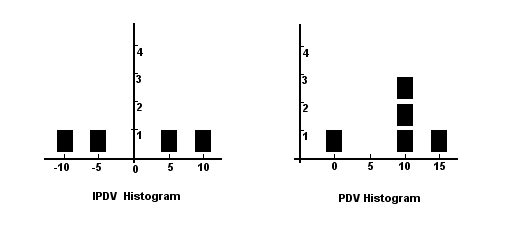
\includegraphics{img/ipdv_pdv.png}}
        \caption{Histogram IPDV a~PDV.}
        \label{pic_delay_histogram}
    \end{center}
\end{figure}

\newpage

Je dokázané, že stredná hodnota IPDV sa blíži alebo je rovná nule, viď 
\cite{rfc_delay_variation_metric_2}. Preto, ak chceme zistiť rozptyl oneskorenia,
ktorý by sme chceli porovnať s~hodnotou uvedenou v~SLA, musíme použiť algoritmus
PDV. 

Nevýhodou algoritmu IPDV je, že v~toku paketov s~veľkou
stratovosťou určí hodnotu rozptylu za neurčitú.
Preto je jeho použitie v~tomto prípade obmedzené.
Aj pre všetky nevýhody IPDV sa používa v~protokole
RTP v~mierne upravenej forme. Je to kvôli schopnosti rýchlejšie reagovať
a~ovplyvniť veľkosti zásobníkov dát \cite{rfc_rtp}.

Pre meranie tohto parametra sieťového prenosu je taktiež nutná dostatočná
synchronizácia času. Problémy spojené s~meraním sú rovnaké ako pri jednosmernom
oneskorení.
Pre správnu implementáciu je taktiež nutné použiť architektúru
klient\,--\,server.

\section{Priepustnosť (throughput)} \label{bandwith}
Tento parameter sieťového prenosu je veľmi dôležitý a~často býva uvedený
SLA od poskytovateľa pripojenia. Podľa
tohto parametra sa riadi väčšina bežných užívateľov pri výbere pripojenia
k~internetu. Priepustnosť môžeme definovať ako maximálnu rýchlosť prenosu
daného objemu dát, pri ktorej nedochádza k~strate alebo zahadzovania
rámcov z~daného toku za jednotku času \cite{rfc_bench_term}.

Nástroje, ktoré dokážu odmerať tento parameter prenosu, musia byť architektúry
klient\,--\,server. Klient generuje a~následne posiela dáta na adresu servera,
ktorý slúži ako prijímajúca stanica, kde sa vytvárajú štatistiky o~prenose.

\subsection{Meranie TCP priepustnosti podľa RFC 6494}
    Dokument RFC 6494 \cite{rfc_tcp_throughput} od skupiny IPPM uvádza,
    že pre koncového užívateľa nie je dôležitá informácia o~výkone siete
    na druhej alebo tretej vrstve internetového modelu TCP/IP, ale 
    reálne dosiahnuteľný výkon s~použitím transportného protokolu 
    TCP \cite{rfc_tcp_throughput}. Je to zapríčinené tým, že väčšina služieb,
    ktoré využívajú koncoví užívatelia, pracuje s~transportným protokolom TCP.
    Meranie TCP priepustnosti je zložitejší proces. Dokument \cite{rfc_tcp_throughput}
    popisuje celú metodiku merania. Pre našu prácu je dôležité si uvedomiť len
    základný princíp merania. Metodika pre svoju činnosť potrebuje zistiť
    viaceré parametre sieťového prenosu:

    \begin{itemize}
        \item Odmerať RTT.
        \item Zistiť veľkosť PMTU.
        \item Odmerať priepustnosť siete na L3 vrstve.
    \end{itemize}

    Meranie RTT môže byť prevedené spôsobom, že sa odmerá
    čas medzi poslaním prvého SYN paketu až po príjem nadväzujúcej odpovede 
    SYN+ACK. Priepustnosť siete môžeme odmerať nástrojom Iperf v~UDP móde, alebo 
    použiť metodiku z~RFC 2544 \cite{rfc_2544}.

    Pojem \emph{PMTU (Path Maximum Transmission Unit)} znamená veľkosť
    maximálnej prenosovej jednotky z~jednej koncovej stanice na druhú, ktorá 
    nebude v~prípade použitia sieťového protokolu IPv4 fragmentovaná. Proces
    zisťovania PMTU sa nazýva \emph{Path MTU Discovery} a~je popísaný
    v~dokumente RFC 1191 \cite{rfc_ipv4_pmtud} pre IPv4 a~v~RFC 1981
    \cite{rfc_ipv6_pmtud} pre IPv6. 

    Transportný protokol pracuje v~troch režimoch: pomalý štart, predchádzanie
    zahltenia a~zotavenie po výpadku. Uvedená metodika sa venuje meraniu výkonu 
    práve v~druhej fáze\,--\,predchádzanie zahltenia, kedy je prenos vo vyváženom 
    stave. Rýchlosť v~tejto fáze dosahuje optimálne hodnoty.

\section{Strata paketov} \label{loss}
Dôležitý parameter sieťového prenosu je strata paketov. Dochádza k~nemu najmä
pri preťažení linky, keď sa zaplnia vstupné rady sieťových zariadení.
K~zahadzovaniu dochádza taktiež pri poškodených rámcoch.

Tento parameter je možné odmerať pomocou transportného protokolu UPD. Protokol TCP
implementuje spoľahlivý prenos, takže nie je možné zistiť z~vyššej vrstvy
modelu OSI, že došlo k~strate paketu. 

Zistenie straty paketov je dôležité pre správnu funkčnosť sieťového prenosu.
Ak prenos prebieha pod
transportným protokolom TCP, dochádza automaticky k~znovu odoslaniu paketu. Pri strate
paketov nesúcich streaming videa alebo iné multimediálne dáta bežiace v~reálnom
čase pod protokolom UDP nedochádza k~znovu odoslaniu. Tým pádom sa zhoršuje
kvalita obrazu alebo zvuku. Preto je nutné pri prenosoch v~reálnom čase
dodržiavať hraničné hodnoty straty a~oneskorenia paketov, aby bol obraz a~zvuk pre
užívateľa dostatočne kvalitný.

\noindent Metodika na zistenie straty paketu, prevzatá z~\cite{rfc_one_way_loss}: 
\begin{enumerate}
    \item Synchronizácia času zdroja a~cieľa.
    \item Výber IP adresy oboch koncových staníc.
    \item Príprava cieľa na príjem paketov.
    \item Zdroj pošle paket s~časom odoslania.
    \item Cieľ príjme paket a~označí ho ako doručený.
    \item Ak cieľ neprijme paket v~rozumnej časovej perióde, 
        označí ho za stratený. Algoritmus sa opakuje od bodu 4.
        pre vopred určený počet paketov.
\end{enumerate}

\section{Zmena poradia paketov} \label{reorder}
K~zmene poradia paketov môže dochádzať napríklad dôsledkom rôznej cesty
jednotlivých paketov alebo zmenou poradia v~zásobníkoch smerovačov 
\cite{rfc_reorder}. 
Multimediálne prenosy v~reálnom čase sú príkladom, kedy je podstatné doručovanie 
datagramov v~správnom poradí.

Nástroje, ktoré dokážu identifikovať zmenu poradia paketov, pracujú
s~transportným protokolom UDP. Použitie TCP nie je možné, tak isto ako v~prípade
diagnostiky straty paketov, pretože implementuje spoľahlivý prenos.

Aby bolo možné identifikovať zmenu poradia, je nutné, aby každý UDP datagram
obsahoval sekvenčné číslo, ktoré jednoznačné určuje poradie. Ak sa príjme paket
so~sekvenčným číslom menším ako posledný prijatý, došlo k~zmene poradia.

\newpage 

\section{Prínos pre našu prácu} \label{parametre_prinos}
Hlbšia znalosť parametrov siete, ktoré charakterizujú výkonnosť, je pre našu
prácu veľmi dôležitá. Testovanie nástrojov na diagnostiku sieťového prenosu 
vyžaduje vytvoriť metodiku, ktorej obsahom bude sledovanie týchto parametrov.
Aby sme chápali princípom merania, bolo nutné tieto metodiky uviesť. Taktiež 
lepšie pochopíme architektúru testovaných nástrojov a~ich softvérové 
nároky, ako je napríklad synchronizácia času. Naštudovanie metodiky malo aj
nemalý prínos z~dôvodu tvorby metodiky samotnej. Takto sme zistili, akým spôsobom
sa tvorí a~všetky náležitosti s~tým spojené. Znalosti použijeme pri tvorbe metodiky
na testovanie nástrojov.

\chapter{Metodika testovania nástrojov} \label{metodika}
Pred samotným testovaním nástrojov je nutné sa zamyslieť, ako túto
činnosť budeme robiť. Je dôležité, aby nástroje boli otestované jednotným 
spôsobom. Takto zaručíme, že ich budeme môcť medzi sebou jednoznačne porovnať.

Väčšina nástrojov bola vyvinutá za účelom odmerať
špecifický parameter sieťového prenosu alebo súbor parametrov. Našou úlohou 
je zvoliť množinu parametrov, ktoré budú skúmané u~každého nástroja.
Samotné parametre na diagnostiku sú najpodstatnejšie, je však 
nutné sa zamyslieť nad vlastnosťami nástrojov, ktoré sú podstatné pri
testovaní a~použiteľnosti pre bežného užívateľa. Medzi tieto doplnkové
vlastnosti patrí napríklad podpora rôznych operačných systémov a~sieťového
protokolu IPv6.

\section{Výber sledovaných parametrov sieťového prenosu} \label{metodika_parametre}
Merateľné parametre sieťového prenosu uvedené v~kapitole \ref{parametre} budú 
predmetom testovania u~každého nástroja na diagnostiku sieťovej komunikácie.
Tieto parametra patria medzi základné vlastnosti sieťového prenosu. Ak by sme sa 
rozhodli bližšie špecifikovať výkonové vlastnosti siete, museli by sme testovanie 
spúšťať pre rôzne veľkosti datagramov, pretože malé datagramy ovplyvňujú výkon procesora
a~naopak veľké priepustnosť aktívnych sieťových zariadení.
Hlavným cieľom našej práce je vytvoriť doporučenie pre bežného užívateľa na
testovanie parametrov sieťového prenosu, takže
musíme vybrať súbor parametrov, ktoré budú reflektovať požiadavky týchto užívateľov.

\noindent Zoznam vybraných parametrov:
\begin{itemize}
    \item TCP priepustnosť
    \item UDP priepustnosť
    \item Oneskorenie
    \item Rozptyl oneskorenia
    \item Zmena poradia paketov
    \item Strata paketov
\end{itemize}

Do zoznamu boli zaradené aj špecifickejšie parametre ako je rozptyl oneskorenia
a~zmena poradia paketov. Budú sledované, ak by sa rozhodli testovať parametre
siete aj skúsenejší užívatelia. 

\section{Výber ďalších funkcionálnych vlastností} \label{metodika_vlastnosti}
Ďalšie parametre alebo vlastnosti nástrojov, ktoré budeme testovať, by mali obsahovať
vlastnosti, ktoré robia nástroj použiteľný na rôznych operačných systémoch,
alebo umožňujú použitie sieťového protokolu IPv6.
Taktiež je vhodné sledovať, či sa daný
nástroj ďalej vyvíja pre podporu do budúcnosti.  

Do testu podpory operačných systémov patria: Windows, Linux
a~FreeBSD. Bežní užívatelia sa budú predovšetkým zaujímať o~podporu
operačného systému Windows a~Linux.

Ďalšou sledovanou vlastnosťou je podpora sieťového
protokolu IPv6 a~správne pracovanie, ak klientská časť nástroja bude
umiestnená za preklad adries.

\noindent Zoznam prídavných sledovaných vlastností nástrojov:
\begin{itemize}
    \item Podpora operačného systému Windows.
    \item Podpora operačného systému Linux.
    \item Podpora operačného systému FreeBSD.
    \item Podpora sieťového protokolu IPv6.
    \item Klient umiestnený za NAT\,--\,om.
\end{itemize}

\section{Metodika testovania}
Po vyčlenení parametrov a~vlastností, ktoré budeme u~každého nástroja 
testovať, je nutné zostaviť systematickú metodiku. Hlavnou úlohou bude
jednoznačne určiť, či nástroj umožňuje alebo implementuje testovanie vyčleneného
parametru sieťového prenosu, alebo či spĺňa dodatočnú funkcionálnu
vlastnosť z~kapitoly \ref{metodika_vlastnosti}. 
Pri testovaní parametrov z~kapitoly \ref{metodika_parametre} nie je 
cieľom metodiky prehlásiť, či sú získané výsledky merania správne.
V~tomto kroku sa nám jedná len o~dokázanie funkcionality.

Testovanie bude prebiehať na skonvergovanej sieti, ktorej topológia nie je 
známa. Dôležité je poznamenať, že prenos môže ovplyvňovať nesprávne
nastavenie sieťových rozhraní, alebo nastavenie operačného systému, ktorý
riadi prenos. Čiže predpokladáme správne nastavenie sieťových rozhraní
koncových staníc, dostatočný výkon a~správne fungovanie softvérového
vybavenia. 

Metodika je rozdelená na dve časti: prvá má za úlohu otestovať parametre 
sieťového prenosu z~kapitoly \ref{metodika_parametre} a~druhá požadované
funkcionálne vlastnosti z~kapitoly \ref{metodika_vlastnosti}. Keďže 
parametrov na testovanie je veľa, v~metodike nebudú uvedené
konkrétne. Overenie podpory sledovaných vlastnosti nástroja by mohlo byť 
urobené na základe naštudovaní manuálových stránok. To však považujeme 
za nepostačujúce a~vlastnosť budeme reálne testovať.
Metodika na meranie parametrov z~kapitoly \ref{metodika_parametre}
má nasledujúci tvar:

\begin{enumerate}
    \item Výber nástroja, ktorý bude predmetom testovania.
    \item Výber \emph{parametru} sieťového prenosu, ktorý chceme testovať.
    \item Preskúmanie manuálových stránok nástroja za učelom zistenie, či
        nástroj implementuje test požadovaného \emph{parametra}. Ak áno,
        metodika pokračuje na ďalší bod. Ak nie, prehlásime, že
        nástroj daný \emph{parameter} nie je schopný odmerať.
    \item Výber dvoch koncových staníc a~určenie IP adries ich sieťových
        rozhraní.
    \item Inštalácia nástroja na zvolených počítačoch.
    \item Spustenie nástroja s~nastavením, aby vykonal 
        test daného \emph{parametra}.
    \item Ak test skončil úspešne a~nástroj zobrazil výsledok v~ľubovoľnej
        forme, môžeme prehlásiť, že nástroj implementuje meranie zvoleného
        \emph{parametra}. Ak výsledok nebol zobrazený, prehlásime, že
            nástroj testovanie \emph{parametra} neimplementuje.
\end{enumerate}

Testovanie požadovaných vlastností nástrojov z~kapitoly
\ref{metodika_vlastnosti} je rozdelené na viacero časti. Prvá sa zameriava
na testovanie podpory operačných systémov, druhá na otestovania sieťového
protokolu IPv6 a~posledná bude mať za cieľ overiť podporu klienta za
prekladom adries.

\noindent Testovanie podpory operačného systému:
\begin{enumerate}
    \item Výber nástroja a~operačného systému, ktorý je predmetom testovania.
    \item Inštalácia nástroja na vybranom operačnom systéme.
    \item Ak sa inštalácia nepodarí, prehlásime nevhodnosť nástroja na daný 
        operačný systém.
    \item Odmeranie ľubovoľného parametra sieťového prenosu. 
    \item Ak sa meranie úspešne dokončilo, nástroj podporuje
        operačný systém.
        V~opačnom prípade
        prehlásime nevhodnosť nástroja na daný operačný systém. 
\end{enumerate}

Podporu sieťového protokolu IPv6 otestujeme spôsobom, že vyberieme jeden
z~už otestovaných parametrov, ktorý nástroj podporuje pre IPv4, a~následne
spustíme test s~adresou IPv6. Prípadne použijeme prepínač na voľbu protokolu IPv6.
Samozrejme, musíme zabezpečiť IPv6 konektivitu oboch testovacích staníc.

Podporu umiestnenia klienta za preklad adries otestujeme
spôsobom, že klientskú časť nástroja umiestnime za NAT a~spustíme test pre
už overený parameter sieťového prenosu.

\section{Zhrnutie}
Vytvorená metodika nám poskytuje ucelenú formu, pomocou ktorej bude možné nástroje
systematickým spôsobom testovať. Tvorba metodiky nás donútila
k~presnejšiemu určeniu cieľa, ktorý obsahuje výber parametrov 
sieťového prenosu, ktoré budeme sledovať.
V~kapitole \ref{nastroje} budeme postupne
popisovať vybrané nástroje a~testovať ich vlastnosti podľa uvedenej metodiky.

\chapter{Prehľad testovaných nástrojov} \label{nastroje}
V~tejto kapitole sa budeme venovať popisu vybraných softvérových nástrojov,
ktoré nám umožňujú merať rôzne parametre siete. Boli vybraté tie najznámejšie
utility, ktoré boli v~čase tvorby tejto práce dostupné.

U~každého nástroja budú uvedené softvérové nároky, popis 
parametrov a~ukážka vybraných testov. Keďže sa nezameriavame na 
špecifické testovanie každého nástroja, popísaný obsah bude predmetom
nami sledovaných parametrov uvedených v~kapitole \ref{metodika}. Z~tejto
kapitoly budeme aplikovať aj metodiku testovania. Pri každom nástroji
bude uvedená záverečná kapitola s~tabuľkou obsahujúcou zoznam parametrov, 
ktoré sa dajú s~nástrojom merať.

Na záver v~kapitole \ref{nastroje_zhod} bude vyhodnotenie všetkých testovaných
nástrojov. Sledované parametre budú uvedené v~tabuľkách pre prehľadnejší výber
správneho nástroja na dané testovanie.

\section{Nástroj Iperf} \label{iperf}
    Prvý z~testovaných nástrojov je Iperf. Bol vyvinutý ako moderná
    alternatíva pre meranie maximálnej priepustnosti pod transportným 
    protokolom TCP a~UDP.
    Pri spustení v~UDP móde je schopný odmerať rozptyl oneskorenia, stratu
    a~výmenu poradia paketov.
    
    K~tejto konzolovej aplikácii bolo vytvorené grafické rozhranie
    s~názvom \emph{Jperf\footnote{Dostupná na
    \url{http://code.google.com/p/xjperf/}}}
    implementované v~jazyku Java.
    Pre účely testovanie sme zvolili verziu 2.0.5
    \footnote{Dostupná na \url{http://sourceforge.net/projects/iperf/}}.

    Existuje nová implementácie s~názvom \emph{Iperf3}, ktorá však nie je spätne
    kompatibilná. Jej cieľom je dosiahnuť jednoduchú implementáciu
    so zameraním na knižnice tak, aby ju mohli využívať iné programy.

        \subsection{Architektúra}\label{iperf_arch}
        Tento program bol implementovaný princípom klient\,--\,server v~jednom
        spustiteľnom súbore. Podľa parametra musíme špecifikovať, ktorý proces 
        chceme spustiť.
        Klient posiela dáta a~server ich prijíma, tieto úlohy sa však môžu
        so~špecifikovaním parametrov vymeniť. Server je implementovaný konkurentným
        spôsobom, takže obslúži viacero klientov súčasne.
        
        Implementácia prebehla v~jazyku C a~C++ s~využitím rozhrania BSD
        soketov. Pre potreby projektu Iperf bola vyvinutá knižnica DAST v~jazyku C++
        viď \cite{iperf_dast}.

        \subsection{Softvérové nároky} \label{iperf_sw}
        Iperf je multiplatformová aplikácia spustiteľná na unixových systémoch
        FreeBSD, Solaris, Linux a~MacOS X. Taktiež je ju možné používať
        na Windows.

        Vo väčšine distribúciach Linuxu je obsiahnutý v~balíčkových
        repozitároch, čo značne uľahčuje inštaláciu a~dostupnosť. 
        Pre priamu kompiláciu zo zdrojových textov je nutné mať nainštalovaný
        gcc a~knižnicu glibc. 
        Grafická nadstavba Jperf je implementovaná v~jazyku Java. Pre jej beh
        je nutné zabezpečiť virtuálne prostredie Java aplikácii (JRE).

        \subsection{Popis vybraných parametrov} \label{iperf_param}
        Jednotlivé parametre nástroja sú uvedené v~tabuľke
        \ref{tab_iperf_parametre}. Tabuľka je rozdelená do niekoľkých častí, aby 
        združila sémanticky podobné prepínače. Iperf je architektúry
        klient\,--\,server implementovaný v~jednom spustiteľnom súbore. Preto 
        je nutné pomocou prepínačov vybrať správny mód.

        \begin{table}[h!]
            \begin{center}
                \begin{tabular}{|l|p{9.2cm}|}
                    \hline
                     \textbf{Parameter}  &  \textbf{Popis}  \\
                    \hline
                    \multicolumn{2}{|c|}{Základné} \\ 
                    \hline
                    -h, \,--\,help     &   výpis nápovedy \\ 
                    -v, \,--\,version   &  výpis verzie  \\
                    -s              &  mód servera \\
                    -c \textless doména\textgreater &  mód klienta,
                        doména špecifikuje adresu
                        alebo doménové meno, na ktorom beží server\\
                    -D, \,--\,deamon   &  spustí server na pozadí \\
                    \hline
                    \multicolumn{2}{|c|}{Nastavenie spojenia} \\ 
                    \hline
                    -p, \,--\,port \textless číslo\textgreater  &
                        špecifikácia portu\\ 
                    -V                  &  použije protokol IPv6 \\
                    -u, \,--\,udp       &  použije UDP protokol namiesto TCP\\
                    -b, \,--\,bandwith \textless číslo\textgreater[KM]  &
                        použitie iba s~-u, bude testovať
                        do maximálnej priepustnosti (implicitne 1 Mbit/s) \\
                    -P, \,--\,parallel \textless číslo\textgreater &
                        vytvorí paralelné testovacie spojenia\\ 
                    \hline
                    \multicolumn{2}{|c|}{Špecifikácia výpisov} \\ 
                    \hline
                    -f, \,--\,format [kmKM] &
                        nastaví jednotky výpisu: Kbits, Mbits,
                        KBytes, MBytes \\
                    -i, \,--\,interval \textless číslo\textgreater &
                        periodické výpisy výsledkov v~sekundách\\
                    -m, \,--\,print\_mss  & vypíše TCP maximum segment
                        size\,--\,MSS a~MTU \\
                    \hline
                    \multicolumn{2}{|c|}{Nastavenie dĺžky trvania testu} \\
                    \hline
                    -t, \,--\,time \textless číslo\textgreater &
                        dĺžka prenosu dát v~sekundách (implicitne 10 s)\\
                    -n, \,--\,num \textless číslo\textgreater[KM] &
                        veľkosť bajtov na prenos (namiesto parametra -t)\\ 
                    \hline
                    \multicolumn{2}{|c|}{Nastavenie prenášaných dát} \\
                    \hline
                    -F, \,--\,fileinput \textless cesta\textgreater &
                    prenášane dáta zoberie zo súboru\\
                    -I, \,--\,stdin   &  prenášane dáta zoberie zo štandardného
                        vstupu\\
                    \hline
                    \multicolumn{2}{|c|}{Obojsmerné testovanie} \\
                    \hline
                    -d, \,--\,dualtest    &  obojsmerný test v~súčasnom čase\\ 
                    -r, \,--\,tradeoff    &  obojsmerný test individuálne \\
                    \hline
                \end{tabular}
                \caption{Vybrané prepínače nástroja Iperf.} 
                \label{tab_iperf_parametre}
            \end{center}
        \end{table}

        \newpage

        \noindent Spustenie klientskej a~serverovej časti:
        \begin{flushleft}
            \texttt{\$ iperf -c <adresa>} \\
            \texttt{\$ iperf -s} 
        \end{flushleft}

        \subsection{Ukážka testov} \label{iperf_testy}
        Pred samotným začatím testovania je potrebné spomenúť, že Iperf
        implicitne spúšťa testovanie TCP priepustnosti na desať sekúnd.

        Obrázok \ref{iperf_s} ukazuje spustenie a~výpis servera bez pridaných
        prepínačov. Na ukážke je naviazané jedno spojenie
        s~identifikačným číslom 4 na test TCP priepustnosti. 
        Výstup poskytuje informácie o~časovej dĺžke testu, množstve 
        prenesených dát a~nameranej priepustnosti. V~tomto 
        prípade klientská strana poskytuje tie isté informácie.

        \begin{figure}[H]
            \begin{center}
                    \scalebox{0.9}{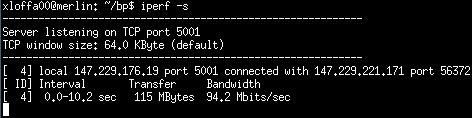
\includegraphics{img/iperf_tcp_prenos.png}}
                \caption{Spustenie a~výpis Iperf servera.}
                \label{iperf_s}
            \end{center}
       \end{figure}

       Pre spustenie klienta je potrebné vedieť doménové meno alebo IP adresu
       hostiteľa, na ktorom beží Iperf server. Zadáva sa ako parameter prepínača 
       \texttt{-c}. 
       Obrázok \ref{iperf_c_i} zobrazuje spustenie klienta
       s~parametrom, ktorý spôsobí periodický výpis nameraných dát. Ako je
       z~obrázku vidieť, bol spustený test na TCP priepustnosť. Keďže sme
       nešpecifikovali dĺžku trvania, test bol spustený na desať sekúnd
       s~periodickými výpismi každé 2 sekundy.

        \begin{figure}[H]
            \begin{center}
                    \scalebox{0.9}{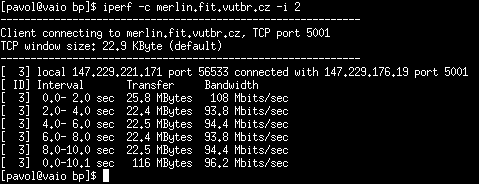
\includegraphics{img/iperf_client_tcp_i.png}}
                \caption{Spustenie a~výpis Iperf klienta pre testovanie TCP
                    priepustnosti.}
                \label{iperf_c_i}
            \end{center}
       \end{figure}

       Pri UDP testovaní musíme špecifikovať maximálnu priepustnosť, ktorú
       chceme testom dosiahnuť, pretože implicitne sa zaháji testovanie do 
       hodnoty 1 Mbps. Pomocou parametra \texttt{-b} môžeme špecifikovať
       hodnotu maximálnej priepustnosti, ktorú chceme otestovať.
       Výstup programu pre UDP testovanie nám poskytuje tie isté informácie ako 
       TCP test, ale je doplnený o~informácie zaslané serverom. 
       Tie zahŕňajú počet stratených
       paketov k~celkovému počtu, rozptyl oneskorenia a~počet paketov prijatých
       v~nesprávnom poradí.
       
       Nasledujúce spustenie klienta pre UDP testovanie ukazuje obrázok 
       \ref{iperf_c_u_i_b_80}. V~tomto meraní sme sa snažili overiť, či je
       možné dosiahnuť na linke priepustnosť 20 Mbps. Ako demonštruje výstup
       programu, linka nie je schopná prenosu na tejto rýchlosti. Ďalej je možné
       dedukovať, že dochádzalo k~výraznej strate paketov. Nastáva tu 
       situácia, v~ktorej sme špecifikovali hornú hranicu testovanej
       priepustnosti väčšiu, ako je reálna. 
       Z~ukážky vidieť, že klient ukazuje priepustnosť 19.7
       Mbps a~server 3.27 Mbps. Hodnoty sa výrazne líšia, presnejšia
       hodnota nameranej priepustnosti je samozrejme od strany servera, pretože
       ten má informácie o~prijatých paketoch, ktoré skutočne prišli.
       Z~tohoto chovania môžeme dedukovať, že server neposkytol informácie
       o~prenesených paketoch klientovi po riadiacom kanáli po skončení testu.

       \begin{figure}[H]
           \begin{center}
                   \scalebox{0.9}{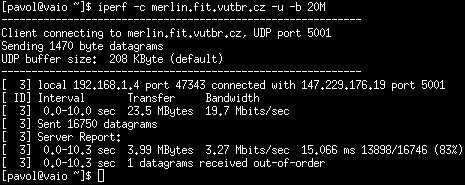
\includegraphics{img/iperf_c_u_b_20_z_domu.png}}
               \caption{Spustenie a~výpis Iperf klienta pre UDP test.}
               \label{iperf_c_u_i_b_80}
           \end{center}
       \end{figure}

        \subsection{Nekorektné správanie} \label{iperf_chyby}
        Na obrázku \ref{iperf_c_u_i_b_80} z~výstupu programu Iperf pri UDP
        testovaní je možné vidieť, že bol prijatý jeden paket v~nesprávnom
        poradí. Toto chybové hlásenie sa vyskytuje vždy, ak zahájime UDP test
        s~priepustnosťou väčšou ako je 3 Mbit/s\,--\,parameter \texttt{-b 3M}.
        Niekedy sa nezobrazí výstup s~informáciami o~UDP priepustnosti, ktoré 
        posiela server klientovi, takže zobrazená priepustnosť je iba
        z~klientovej strany, ktorá môže obsahovať nesprávne informácie.

        \subsection{Zhodnotenie} \label{iperf_zhod}
        Pre meranie základných parametrov siete ako je priepustnosť, rozptyl 
        oneskorenia a~stratovosť paketov je Iperf vhodný nástroj. 
        Poskytuje veľmi jednoduché ovládanie a~je dostupný pre väčšinu dnes
        používaných systémov. 

        Ako ďalšie kladne hodnotiace fakty musíme spomenúť použitie obojstranných
        testov a~možnosť emulovať paralelne testovacie spojenia medzi jednou
        inštanciou klienta a~servera.
        Taktiež schopnosť serveru obslúžiť súčasne viacerých klientov 
        (konkurentný server). Dôležitým faktom je funkčnosť protokolu IPv6 pre 
        budúce použitie tohto nástroja.

        Za výrazný nedostatok považujeme fakt, že server pracuje iba v~jednom zo zvolených
        módov a~to TCP alebo UDP. Pre testovanie z~jednej stanice pomocou TCP
        a~UDP je potreba spustiť dve rôzne inštancie servera.

        Tabuľka \ref{tab_iperf_param} poskytuje súhrnné informácie o~možností
        použitia nástroja Iperf na meranie parametrov sieťového prenosu. Ďalšia
        tabuľka \ref{tab_iperf_vlast} obsahuje informácie o~dodatočných
        vlastnostiach tohto nástroja.

        \begin{table}[H]
            \begin{center}
                \begin{tabular}{|c|c|c|c|c|c|}
                    \hline
                    \textbf{TCP priep.}  &  \textbf{UDP priep.}  &
                    \textbf{Oneskorenie} & \textbf{Jitter} &
                    \textbf{Zmena poradia} & \textbf{Strata} \\
                    \hline
                    $\surd$ & $\surd$ &  & $\surd$ &  & $\surd$ \\ 
                    \hline
                \end{tabular}
                \caption{Merateľné parametre siete nástroja Iperf.}
                \label{tab_iperf_param}
            \end{center}
        \end{table}

        \begin{table}[H]
            \begin{center}
                \begin{tabular}{|c|c|c|c|c|} 
                    \hline
                    \textbf{Linux}  &  \textbf{Windows}  &
                    \textbf{FreeBSD} & \textbf{IPv6} &
                    \textbf{NAT} \\
                    \hline
                    $\surd$ & $\surd$ &  & $\surd$ & $\surd$ \\ 
                    \hline
                \end{tabular}
                \caption{Ďalšie vlastnosti nástroja Iperf.}
                \label{tab_iperf_vlast}
            \end{center}
        \end{table}

  \section{Nástroj Netperf} \label{netperf}
    Ďalším vybraným nástrojom je Netperf. Je to testovací nástroj na meranie 
    rôznych aspektov sieťového výkonu \cite{netperf_manual}.
    Primárne určený na jednosmerné testovanie prenosu pod protokolom TCP, UDP
    a~SCTP. Oproti aplikácii Iperf je s~ním možné testovať rôzne špecifickejšie 
    vlastnosti sieťového prenosu.
    Je implementovaný ako konzolová aplikácia.
    Pre účely testovania bola vybraná verzia 2.6.0
    \footnote{Dostupná na \url{http://www.netperf.org/netperf/}}.

        \subsection{Architektúra}\label{netperf_arch}
        Architektúra nástroja Netperf je založená na modely klient\,--\,server.
        Nástroj je rozdelený do dvoch spustiteľných programov \texttt{netperf}
        a~\texttt{netserver}, ktorý reprezentuje serverovú časť.

        Ako u~nástroja Iperf, klient generuje dátový prenos a~server 
        prijíma na danom porte. Každé spojenie medzi klientom
        a~serverom obsahuje dva komunikačné kanály, na jednom sa 
        prenášajú riadiace informácie a~druhý slúži na
        prenos testovaných dát.
        Implementácia prebehla v~jazyku C s~použitím rozhrania BSD soketov.

        \subsection{Softvérové nároky} \label{netperf_sw}
        Tento nástroj je taktiež multiplatformová aplikácia spustiteľná na
        pomerne všetkých dostupných operačných systémoch. Patria tu unixové
        operačné systémy, Linux a~FreeBSD, ale aj operačný systém Windows.

\newpage

        \subsection{Popis vybraných parametrov} \label{netperf_param}
        Tabuľka \ref{tab_netperf_parametre} obsahuje vybrané parametre, ktoré sú
        predmetom testovania nami skúmaných parametrov sieťového prenosu. Taktiež sú zlúčené 
        podľa sémanticky podobných vlastností.

        \begin{table}[H]
            \begin{center}
                \begin{tabular}{|l|p{11cm}|}
                    \hline
                     \textbf{Parameter}  &  \textbf{Popis}  \\
                    \hline
                    \multicolumn{2}{|c|}{Základné} \\
                    \hline
                    -h  &  výpis nápovedy \\ 
                    -V  &  výpis verzie  \\
                    -D  &  spustí server na popredí \\
                    \hline
                    \multicolumn{2}{|c|}{Nastavenie spojenia} \\
                    \hline
                    -p \textless číslo\textgreater &  
                        špecifikácia čísla portu\\ 
                    -4   &  použije IPv4 adresu, nastaví AF\_INET \\
                    -6   &  použije IPv6 adresu, nastaví AF\_INET6 \\
                    -t \textless typ\textgreater  & 
                           typ transportného protokolu, pre UDP hodnota
                           UDP\_STREAM, pre TCP TCP\_STREAM (implicitné)\\
                    \hline
                    \multicolumn{2}{|c|}{Špecifikácia výpisov} \\
                    \hline
                    -f \textless [GMKgmk]\textgreater & 
                        nastaví jednotky výpisu, veľké písmena umocnia
                        jednotky na druhú a~malé na desiatu\\
                    \hline
                    \multicolumn{2}{|c|}{Nastavenie dĺžky trvania testu} \\
                    \hline
                    -l \textless číslo\textgreater &
                        dĺžka prenosu dát v~sekundách (implicitne 10 s)\\
                    \hline
                    \multicolumn{2}{|c|}{Nastavenie prenášaných dát} \\
                    \hline
                    -F \textless cesta\textgreater & 
                        prenášane dáta zoberie zo súboru \\
                    \hline
                    \multicolumn{2}{|c|}{Test špecifické} \\
                    \hline
                    -m \textless číslo\textgreater &
                        nastavenie veľkosti poľa predávaného
                        funkcii send, nemusí priamo ovplyvniť veľkosť
                        posielaného paketu, použitie pri UDP\_STREAM\\
                    -s \textless číslo\textgreater  & 
                        nastaví veľkosť prijímajúceho
                        a~odosielaného poľa na strane klienta.\\
                    -S \textless číslo\textgreater &
                        nastaví veľkosť prijímajúceho
                        a~odosielaného poľa na strane servera.\\
                     \hline
                \end{tabular}
                \caption{Vybrané prepínače nástroja Netperf.} 
                \label{tab_netperf_parametre}
            \end{center}
        \end{table}

        \noindent Parametre sa vo všeobecnosti delia na globálne a~test špecifické.
        Test špecifické musia byť oddelené dvoma znakmi "-". 
        Uvádzame príkaz na základné spustenie klienta a~servera:
        \begin{flushleft}
            \texttt{\$ netperf -H <adresa,protokol> -p <port> <globálne> -- <test špecifické>} \\
            \texttt{\$ netserver <adresa,protokol> -p <port> -D}
        \end{flushleft}
        \noindent Protokol sa špecifikuje číslom 4 pre IPv4 (AF\_INET) a~6 pre 
        IPv6 (AF\_INET6). Je to nepovinná položka. Ak sa nezadá,
        použije sa AF\_UNSPEC.

        \subsection{Ukážka testov} \label{netperf_testy}
        V~tejto sekcii sa pozrieme na možné testy s~nástrojom Netperf.
        Pri spustení bez parametrov upravujúcich testovanie sa zaháji
        implicitne prenos nad transportným protokolom TCP na dĺžku trvania
        desať sekúnd. 

        Pre úspešné testovanie je potrebné zabezpečiť beh
        inštancie \texttt{netserver} na hostiteľovi, na ktorý sa budú
        generovať dáta z~klientskej časti \texttt{netperf}.
        Aplikácia \texttt{netserver} nevypisuje žiadne výpisy. Pri štandardnom spustení sa spustí
        na pozadí. Toto chovanie môžeme potlačiť parametrom \texttt{-D}. Keďže
        serverová aplikácia neposkytuje žiadne samostatne výpisy, nebude
        uvádzať terminálové obrázky z~jej behu.

        Klientská časť vyžaduje jeden povinný prepínač \texttt{-H}, ktorý
        vyžaduje parameter doménové meno, alebo IP adresu hostiteľa, na
        ktorom beží server.

        Prvý test môžeme vidieť na obrázku \ref{netperf_l_90}, na ktorom
        je uvedený výstup pri testovaní priepustnosti pod transportným
        protokolom TCP. Výstup aplikácie pri
        tejto konfigurácii poskytuje informácie o~maximálne dosiahnutej
        priepustnosti, dĺžke trvaní testu a~veľkosti zásobníkov pre 
        príjem a~odoslanie dát. Výpis taktiež poskytuje informáciu 
        o~veľkosti posielanej správy. Z~obrázka \ref{netperf_l_90} vyplýva, že
        bola dosiahnutá priepustnosť 93,7 Mbit/s.

       \begin{figure}[H]
           \begin{center}
                   \scalebox{0.7}{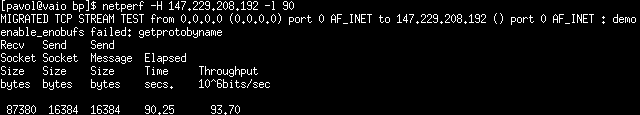
\includegraphics{img/netperf_client_l_90.png}}
               \caption{Spustenie a~výpis nástroja Netperf pre TCP\_STREAM.}
               \label{netperf_l_90}
           \end{center}
       \end{figure}

       Následujúci test z~obrázku \ref{netperf_ipv6_udp} demonštruje spustenie
       klienta, ktorý zaháji testovanie pod transportným protokolom UDP. Táto
       možnosť bola dosiahnutá prepínačom \texttt{-t UDP\_STREAM}. Názorne
       môžeme vidieť použitie IPv6 adresy hostiteľa, na ktorej beží serverová
       časť. Takto sa použil sieťový protokol IPv6 bez ďalších prídavných 
       prepínačov.

       Výstup nám poskytuje informácie o~dosiahnutej priepustnosti, dĺžke
       trvania, ale aj počet chybne a~správne prenesených správ. Ako demonštruje
       obrázok, posledné dva riadky obsahujú namerané výsledky, ktoré nie sú
       totožné. Posledný riadok je výstup nameraných údajov \texttt{netserveru}, ktorý
       po ukončení testu poslal dáta klientovi. Údaje nie sú totožné, pretože
       bolo odoslané väčšie množstvo dát, aké bolo prijaté serverom. Toto je
       typický fakt pri testovaní pod transportným protokolom UDP, dáta je možné
       rýchlejšie odoslať, ale nie všetky budú korektne prijaté. Môžeme vidieť,
       že počet prijatých správ na servery bol menší ako odoslaných.

      \begin{figure}[H]
           \begin{center}
                   \scalebox{0.7}{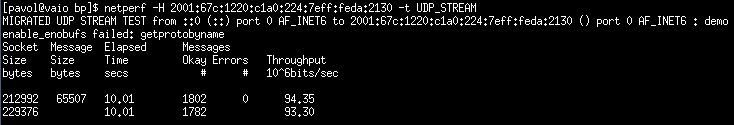
\includegraphics{img/netperd_client_ipv6_udp.png}}
               \caption{Spustenie a~výpis nástroja Netperf pre UDP\_STREAM.}
               \label{netperf_ipv6_udp}
           \end{center}
       \end{figure}

        \subsection{Nekorektné správanie} \label{netperf_chyby}
        S~nástrojom Netperf sa nám nepodarilo previesť testovania pod protokolom
        UDP a~spojazdniť komunikáciu so sieťovým protokolom IPv6. Obe tieto 
        vlastnosti sú v~nástroji implementované a~uvedené v~manuálových
        stránkach. Testovanie pod transportným protokolom UDP sa podarilo 
        spojazdniť pri použití rovnakých operačných systémoch na koncových
        staniciach. Utilita však nechcela nadviazať spojenie pomocou IPv4.
        Preto meranie UDP priepustnosti nepovažujeme za správne fungujúce.

        \subsection{Zhodnotenie} \label{netperf_zhod}
        Medzi hlavné výhody tohto konzolového nástroja považujeme úplne
        ovládanie servera z~aplikácie klienta. To umožňuje použitie rozličných
        parametrov. Pre plnohodnotné testovanie stačí spustenie jednej inštancie
        servera na vzdialenom hostiteľovi. Toto chovanie je veľmi vhodné,
        pretože nevyžaduje opakované spustenie serverovej časti pri zmene
        transportného protokolu. Aplikácia taktiež poskytuje veľmi zrozumiteľné
        výstupy, ktoré uvádzajú tie najdôležitejšie fakty.

        Za nedostatok môžeme považovať nemožnosť získať informácie
        o~zmene poradia, strate paketov a~hodnote jitter pri
        testovaní pod transportným protokolom UDP. 
        Pomocou filtrácie a~analýzy sieťového toku bolo zistené, že parameter \texttt{-m} 
        nastaví veľkosť dát posielaných v~UDP rámci, avšak nie celkovú veľkosť
        paketu. Ak celková veľkosť presiahne
        MTU, je správa fragmentovaná. Toto správanie uvedeného prepínača musíme 
        pri testovaní brať v~úvahu. 
        Tabuľky \ref{tab_netperf_param} a~\ref{tab_netperf_vlast} obsahujú
        súhrnné informácie o~možnostiach testovania pomocou tohto nástroja.

        \begin{table}[H]
            \begin{center}
                \begin{tabular}{|c|c|c|c|c|c|}
                    \hline
                    \textbf{TCP priep.}  &  \textbf{UDP priep.}  &
                    \textbf{Oneskorenie} & \textbf{Jitter} &
                    \textbf{Zmena poradia} & \textbf{Strata} \\
                    \hline
                    $\surd$ & &  &  &  & \\ 
                    \hline
                \end{tabular}
                \caption{Merateľné parametre siete nástroja Netperf.}
                \label{tab_netperf_param}
            \end{center}
        \end{table}

        \begin{table}[H]
            \begin{center}
                \begin{tabular}{|c|c|c|c|c|}
                    \hline
                    \textbf{Linux}  &  \textbf{Windows}  &
                    \textbf{FreeBSD} & \textbf{IPv6} &
                    \textbf{NAT} \\
                    \hline
                    $\surd$ & $\surd$ & $\surd$ &  & $\surd$ \\ 
                    \hline
                \end{tabular}
                \caption{Ďalšie vlastnosti nástroja Netperf.}
                \label{tab_netperf_vlast}
            \end{center}
        \end{table}

    \section{Nástroj BWCTL} \label{bwctl}
    BWCTL je terminálová aplikácia, ktorá zabezpečuje meranie priepustnosti
    prostredníctvom iných nástrojov. 
    Pre svoju funkčnosť potrebuje niektorý z~nástrojov na
    meranie sieťových parametrov. Medzi tieto nástroje patrí Iperf, Thrulay
    a~Nuttcp. Kombináciou týchto aplikácii pri testovaní je schopný BWCTL
    odmerať široké spektrum sieťových parametrov. Samotná aplikácia
    neimplementuje žiadne testovacie techniky, avšak externe spúšťa uvedené
    nástroje. Takto docielime, že pomocou jednej bežiacej utility na
    servery budeme schopní testovať pomocou troch rozličných nástrojov.

    Úlohou BWCTL bolo taktiež zaviesť prvky, ktoré konkurenčné nástroje
    neobsahovali. Jedná sa o~podporu plánovania a~zabezpečenia. To však nie je 
    predmetom našej práce.
    Pre testovanie sme použili verziu 1.4
    \footnote{Dostupná na \url{http://www.internet2.edu/performance/bwctl/}}.

        \subsection{Architektúra}\label{bwctl_arch}
        Taktiež sa jedná o~aplikáciu klient\,--\,server, takže pre testovanie
        potrebuje spustený ďalší proces na vzdialenom stroji.
        Nástroj sa delí na dve samostatne spustiteľné aplikácie. Prvá slúži na 
        inicializáciu a~nastavovanie parametrov testovania, je to klient
        \texttt{bwctl}.
        Druhá slúži ako
        démon bežiaci na vzdialenom hostiteľovi. Jej názov je \texttt{bwctld}.

        Významnou funkciou je schopnosť spustiť testovanie z~klienta tak, že
        nebude jednou z~koncových staníc. Tento spôsob nám umožňuje
        testovanie medzi sieťovými uzlami, na ktoré nemáme prístup.

        \subsection{Softvérové nároky} \label{bwctl_sw}
        Nároky na softvér tohto nástroja sú obsiahlejšie, pretože pre svoju
        funkčnosť potrebuje iné aplikácie.
        Na stanici, na ktorej budeme chcieť úspešne testovať, musí byť
        nainštalovaný jeden z~nástrojov Iperf, Thrulay alebo Nuttcp.
        Pre úspešné testovanie ďalej vyžaduje, aby koncové stanice mali synchronizovaný
        čas pomocou NTP protokolu, čiže spustený NTP démon.
        Podpora NTP sa dá potlačiť parametrom \texttt{-a}, ale toto
        nastavenie nezaručuje správne výsledky testov. Aplikácia taktiež môže
        skončiť s~chybovým návratovým kódom. 

        Samotný nástroj bol úspešne testovaný na linuxových systémoch 
        s~jadrom verzie 2.4, 2.6 a~FreeBSD 4.X a~5.X.  
        Na systéme Solaris sa nedá úspešne skompilovať Thurlay, takže jeho
        použitie je obmedzené.
        Nástroj nie je dostupný ako balíček v~linuxových distribúciách, preto je 
        potrebné kompilovanie zo zdrojových textov. Kompilácia vyžaduje
        GNU Make.

        \subsection{Popis vybraných parametrov} \label{bwctl_param}
        Väčšina podporovaných prepínačov je prevzatá z~nástroja Iperf,
        ktoré sú uvedené v~tabuľke \ref{tab_iperf_parametre}. Je dôležité si overiť 
        sémantiku  daných prepínačov, pretože sa môžu líšiť.
        Uvedená tabuľka \ref{tab_bwctl_parametre} obsahuje vlastné 
        prepínače tohto nástroja. Jedná sa hlavne o~viacnásobné
        spustenie testovania.
        Démon na strane servera prijíma len určité parametre, viď tabuľka 
        \ref{tab_bwctl_parametre} a~\cite{bwctld_manual}.

        \begin{table}[H]
            \begin{center}
                \begin{tabular}{|l|p{11cm}|}
                    \hline
                     \textbf{Parameter}  &  \textbf{Popis}  \\
                    \hline
                    \multicolumn{2}{|c|}{Základné} \\
                    \hline
                    -h  &  výpis nápovedy \\ 
                    -V  &  výpis verzie  \\
                    -a syncfuzz & povolí testovanie bez NTP démona \\
                    -T \textless program\textgreater & 
                        určí nástroj pre testovanie,
                        možné voľby sú Iperf, Nuttcp, Thrulay \\
                    -f [kmKM] &
                        nastaví jednotky výpisu: Kbits, Mbits,
                        KBytes, MBytes \\
                    \hline
                    \multicolumn{2}{|c|}{Nastavenie spojenia} \\
                    \hline
                    -4   &  použije IPv4 adresu, (implicitne preferuje IPv6)\\
                    -6   &  vynúti použitie IPv6 adresy \\
                    -c \textless adresa\textgreater & adresa alebo 
                        doménove meno stanice, ktorá bude prijímať dáta\\
                    -s \textless adresa\textgreater &  adresa alebo
                        doménove meno stanice, ktorá bude posielať dáta\\
                    \hline
                    \multicolumn{2}{|c|}{Riadenie testovania} \\
                    \hline
                    -I \textless číslo\textgreater & 
                        časový interval v~sekundách v~ktorom bude periodicky
                        spúšťat testovanie \\
                    -n \textless číslo\textgreater & 
                        povolí spustenie určitého počtu testov
                        (použitie s~-I) \\
                    \hline
                    \multicolumn{2}{|c|}{Parametre pre bwctld} \\
                    \hline
                    -c \textless adresa\textgreater & 
                        adresár s~konfiguračnými súbormi \\ 
                    -Z  & spustí server na popredí \\
                    \hline
                \end{tabular}
                \caption{Vybrané parametre nástroja BWCTL.} 
                \label{tab_bwctl_parametre}
            \end{center}
        \end{table}

\newpage

        \noindent Príkaz na spustenie klienta a~démona na popredí:

        \begin{flushleft}
            \texttt{\$ bwctl -c <adresa>} \\
            \texttt{\$ bwctld -Z }
        \end{flushleft}

        \subsection{Ukážka testov} \label{bwctl_testy}
        Testovanie pomocou BWCTL môže byť značne jednoduché, pretože združuje 
        viacero nástrojov, ktoré sú ovládané tým istým rozhraním. 
        Nasledujúci test z~obrázka \ref{bwctl_c_f_k} ukazuje meranie TCP
        priepustnosti. Ako je vidieť, ak pomocou parametra \texttt{-T}
        nešpecifikujeme použitý nástroj, spustí sa meranie pomocou nástroja Iperf 
        pre TCP test s~dĺžkou trvania desať sekúnd. Takto spustený test
        s~parametrom \texttt{-c} spôsobí, že klient bude generovať a~následne
        posielať dáta na server, kde beží \texttt{bwctld} démon, ktorý dáta prijme.
        Ak zvolíme parameter \texttt{-s}, bude prenos dát prebiehať v~opačnom
        smere. 

       \begin{figure}[H]
           \begin{center}
                   \scalebox{0.80}{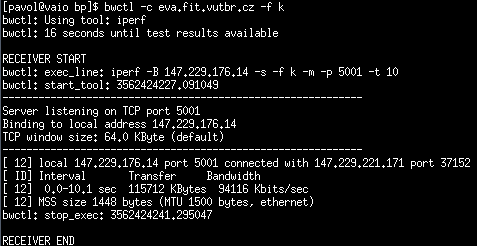
\includegraphics{img/bwctl_c_f_k.png}}
               \caption{Ukážka testu TCP priepustnosti s~použitím nástroja BWCTL.}
               \label{bwctl_c_f_k}
           \end{center}
       \end{figure}

       Využitie schopností nástroja BWCTL ukazuje test na obrázku
       \ref{bwctl_c_f_m_I_10_t_2}. Každých desať sekúnd spustí testovanie
       s~dĺžkou trvania 2 sekundy pomocou nástroja Iperf pre meranie maximálnej
       TCP priepustnosti.

       \begin{figure}[H]
           \begin{center}
                   \scalebox{0.81}{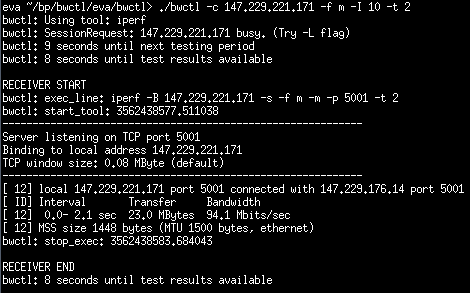
\includegraphics{img/bwctl_c_f_m_I_10_t_2.png}}
               \caption{Ukážka opakovaného spustenia testu pomocou BWCTL.}
               \label{bwctl_c_f_m_I_10_t_2}
           \end{center}
       \end{figure}

        \subsection{Nekorektné správanie} \label{bwctl_chyby}
        Pri testovaní sa vyskytovali problémy pri spustení v~UDP móde. Väčšinou
        nemohlo byť naviazané spojenie. 
        S~prepínačom \texttt{-I} nastávala
        situácia, že klient v~niektorých periódach nemohol naviazať spojenie
        s~démonom na vzdialenej stanici. Vypisovaná hláška bola: \\
        \texttt{SessionRequest: host busy. (Try -L flag)}. 

        \subsection{Zhodnotenie} \label{bwctl_zhod}
        Ako už bolo spomenuté tento nástroj  pre testovanie využíva
        iné programy, takže nám neprináša žiadne
        vylepšenia a~k~výsledkom by sme sa
        dopracovali použitím utilít, ktoré využíva.

        Nevýhodou tohto nástroja je komplikovaná inštalácia, ktorá vyžaduje
        oddelené inštalovanie ďalších nástrojov.
        Ďalší záporný fakt je použitie démona NTP. 

        Ak sa rozhodneme pre dlhodobejšie a~obsiahlejšie testovanie, tento
        nástroj bude správnou voľbou, pretože poskytne jednotné rozhranie pre
        viacero nástrojov, ktoré by sme museli obsluhovať samostatne.

        Tabuľky, ktoré obsahujú súhrnné informácie o~možnostiach testovania
        parametrov siete, neuvádzame, pretože tento nástroj len spúšťa ďalšie 
        aplikácie. Keďže každý z~nástrojov bude otestovaný samostatne. Tabuľky
        uvedieme v~príslušnej kapitole.

    \section{Nástroj OWAMP}
    Tento nástroj neslúži na meranie priepustnosti siete. Implementuje
    protokol \emph{OWAMP (One Way Active Measurement Protocol)}, ktorý slúži na
    meranie času prenosu paketu z~jedného hostiteľa na druhého (jednosmerné
    oneskorenie). Je podobný aplikácii Ping, ktorá sa zameriava na 
    vyhodnotenie času RTT. 
    RTT môžeme chápať ako dvojnásobnú hodnotu času prenosu paketu z~jedného
    hostiteľa na druhého. Týmto dospejeme k~nepresnej hodnote a~tento spôsob nie
    je správny. Kvôli tomu vznikol protokol OWAMP \cite{rfc_owamp}
    a~aplikácia s~rovnakým názvom OWAMP ho implementuje.

    Výstup tejto konzolovej aplikácie nám poskytuje informácie o~časoch
    potrebných na prenesenie paketu z~jedného hostiteľa na druhého v~oboch
    smeroch. 
    Pre účely testovania bola použitá verzia
    3.3\footnote{Dostupná na
    \url{http://www.internet2.edu/performance/owamp/index.html}}.

        \subsection{Architektúra}\label{owamp_arch}
        Nástroj taktiež vychádza z~modelu klient\,--\,server. Aplikácia
        je rozdelená do dvoch samostatne spustiteľných programov.
        Klientská utilita má názov \texttt{owping} a~server \texttt{owampd},
        ktorý sa normálne
        spúšťa na pozadí a~poskytuje minimálne množstvo výpisov.

        \subsection{Softvérové nároky} \label{owamp_sw}
        Má podobné nároky na softvér ako aplikácia BWCTL. Oba sú
        vyvíjané rovnakou organizáciou.
        Vyžaduje synchronizovaný čas pomocou NTP protokolu, čiže spustený
        príslušný démon. Oproti aplikácii BWCTL sa táto požiadavka nedá
        potlačiť prepínačom.

        Podporované operačné systémy sú FreeBSD, MacOS X, Linux a~Solaris. 
        Nástroj je dostupný ako balíček pre niektoré distribúcie Linuxu. Ak je
        potrebná kompilácia zo zdrojových textov, vyžaduje program GNU Make.

        \subsection{Popis vybraných parametrov} \label{owamp_param}
        Podobne ako BWCTL aj tento nástroj obsahuje možnosti zabezpečenia
        a~autentizácie. To však nie je predmetom našej práce, tak sa zameriame 
        len na prepínače súvisiace s~testovaním. Tabuľka 
        \ref{tab_owamp_parametre} obsahuje vybrané prepínače programov
        \texttt{owping} a~\texttt{owampd}.

        \begin{table}[H]
            \begin{center}
                \begin{tabular}{|l|p{11cm}|}
                    \hline
                     \textbf{Parameter}  &  \textbf{Popis}  \\
                    \hline
                    \multicolumn{2}{|c|}{Prepínače pre owping} \\
                    \hline
                    -h      &  výpis nápovedy \\ 
                    -c \textless číslo\textgreater & 
                    počet testovacích paketov, (implicitne 100)   \\
                    -f      &  prevedie jednosmerný test smerom od vzdialeného
                                hostiteľa \\ 
                    -t      &  prevedie jednosmerný test smerom k~vzdialenému
                                hostiteľovi \\ 
                    -s \textless číslo\textgreater & veľkosť paketu\\
                    -4      &  použije IPv4 protokol, (implicitne
                                preferuje IPv6) \\ 
                    -6      &  použije IPv6 protokol \\ 
                    \hline
                    \multicolumn{2}{|c|}{Prepínače pre owampd} \\
                    \hline
                    -Z      &  spustenie na popredí \\ 
                    -c \textless adresa\textgreater  &  
                        cesta k~priečinku obsahujúcemu 
                        konfiguračné súbory (owampd.conf, owampd.limits,
                        ak sa nezadá berie aktuálny pracovný adresár)\\ 
                    -S \textless adresa\textgreater:port & určí
                        adresu a~port na ktorom bude prijímať spojenia\\
                    \hline
                \end{tabular}
                \caption{Vybrané parametre nástroja OWAMP.} 
                \label{tab_owamp_parametre}
            \end{center}
        \end{table}

        \noindent Klient \texttt{owping} vyžaduje jeden povinný parameter\,--\,adresu
        vzdialeného počítača s~bežiacim procesom \texttt{owampd}.
        Spustenie základného testu môže vyzerať nasledovne:

        \begin{flushleft}
            \texttt{\$ owping <adresa>:<port>} \\
            \texttt{\$ owampd -S <adresa>:<port> -Z }
        \end{flushleft}

        V~prípade použitia IPv6 je potrebné uviesť port v~hranatých
        zátvorkách. Parameter \texttt{-Z} spôsoby spustenie démona na popredí.
        Démon je možné spustiť dvoma spôsobmi. Prvý vyžaduje konfiguračný súbor.
        Cesta k~nemu sa zadáva prepínačom \texttt{-c}. Druhý spôsob spustenia 
        sme uviedli v~ukážke.

        V~prípade spustenia s~konfiguračným súborom je nutné upraviť jeden
        riadok v~súbore owampd.conf. Zadáme adresu a~port, na ktorom bude prijímať
        spojenia. Protokol OWAMP má rezervovaný port 861,
        ktorý vyžaduje práva super užívateľa. Pokiaľ chceme toto správanie
        obísť, musíme zvoliť iné číslo.

        \begin{flushleft}
            \texttt{srcnode localhost:861} \\
            \texttt{srcnode eva.fit.vutbr.cz:8611}
        \end{flushleft}

        \subsection{Ukážka testov} \label{owamp_testy}
        Na nasledujúcom teste si ukážeme, ako môžeme odmerať jednosmerné 
        latencie na ceste k~vzdialenej sieťovej stanici.
        Obrázok \ref{owping_c_110} obsahuje výstup z~aplikácie \texttt{owping}. 
        Pomocou parametra \texttt{-c} bol upravený počet testovacích paketov
        z~implicitnej hodnoty 100 na 110.
        Výstup programu obsahuje informácie o~jednosmernom oneskorení v~oboch
        smeroch medzi testovanými stanicami. Medzi ďalšie informácie, ktoré
        poskytuje, patrí počet skokov, rozptyl oneskorenia a~strata paketov.

       \begin{figure}[H]
           \begin{center}
                   \scalebox{0.9}{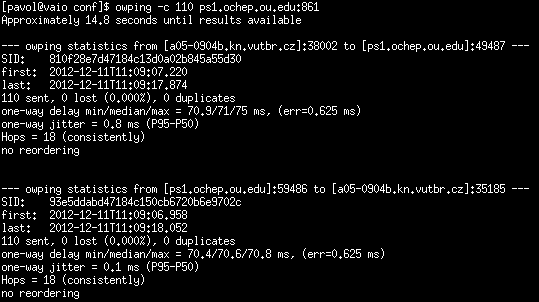
\includegraphics{img/owping_c_110.png}}
                   \caption{Ukážka spustenia nástroja Owping.}
               \label{owping_c_110}
           \end{center}
       \end{figure}

        \subsection{Nekorektné správanie} \label{owamp_chyby}
        Ak sa klient nachádzal za prekladom adries, nebolo možné 
        nadviazať spojenie s~démonom. Z~toho vyplýva, že aplikáciu nebude
        môcť používať väčšina bežných užívateľov kvôli rozšírenému použitiu  
        prekladu adries.

        \subsection{Protokol OWAMP}
        Protokol OWAMP vznikol na požiadavky merania jednosmerného
        oneskorenia. Oproti nástroju Ping má umožňovať aj meranie stratovosti 
        paketov.  
        Protokol poskytuje možnosť merania zo stanice, ktorá nieje 
        ani jednou z~koncových bodov. Takto môžeme testovať 
        oneskorenie medzi stanicami, na ktoré nemáme prístup.
        Medzi ďalšie vlastnosti protokolu patrí autentifikácia 
        koncových bodov.
        
        Pre tieto požiadavky bolo nutné protokol rozdeliť na dve časti:
        ovládaciu a~testovaciu. Prvá má za účel nadviazať spojenie.
        Tieto správy nesú parametre merania a~údaje pre
        autentifikáciu. Správy určené pre testovanie obsahujú časové 
        razítko a~sekvenčné číslo. Kvôli bezpečnostným vlastnostiam protokolu
        môžu obsahovať aj ďalšie údaje, napríklad pre overenie identity.
        Testovacie pakety môžu mať ľubovoľne nastavenú veľkosť.

        \subsection{Zhodnotenie} \label{owamp_zhod}
        Nástroj hodnotíme veľmi kladne. Síce nám neposkytuje funkcionalitu
        v~podobe merania priepustnosti, ale dokáže odmerať rozptyl oneskorenia, stratu
        a~zmenu poriadia paketov. Hlavnou úlohou je určenie jednosmerných
        latencií na linke medzi testovanými zariadeniami. Takto môžeme zistiť,
        že latencie sa môžu na daných smeroch líšiť, taktiež aj počet skokov
        a~iné parametre. Nástroj je jednoduchý na ovládania a~dobre 
        odladený. Tabuľka \ref{tab_owamp_param} obsahuje súhrnné informácie
        o~možnostiach použitia tohto nástroja pri diagnostikovaní siete.
        Tabuľka \ref{tab_owamp_vlast} ukazuje ďalšie vlastnosti
        tohto nástroja.

        Nevýhodu vidíme v~nutnosti použitia démona NTP na
        testovaných staniciach, čo je však pre meranie jednosmerného
        oneskorenia nevyhnutná súčasť správnej implementácie.
        Ak sa klient nachádza za prekladom adries, výrazne znižuje použiteľnosť
        nástroja kvôli implementácii, ktorá toto rozmiestnenie nedovoľuje.

        \begin{table}[H]
            \begin{center}
                \begin{tabular}{|c|c|c|c|c|c|}
                    \hline
                    \textbf{TCP priep.}  &  \textbf{UDP priep.}  &
                    \textbf{Oneskorenie} & \textbf{Jitter} &
                    \textbf{Zmena poradia} & \textbf{Strata} \\
                    \hline
                    & & $\surd$ & $\surd$ &  $\surd$ & $\surd$\\ 
                    \hline
                \end{tabular}
                \caption{Merateľné parametre siete pomocou nástroja OWAMP.}
                \label{tab_owamp_param}
            \end{center}
        \end{table}

        \begin{table}[H]
            \begin{center}
                \begin{tabular}{|c|c|c|c|c|}
                    \hline
                    \textbf{Linux}  &  \textbf{Windows}  &
                    \textbf{FreeBSD} & \textbf{IPv6} &
                    \textbf{NAT} \\
                    \hline
                    $\surd$ & & $\surd$ & $\surd$ &  \\ 
                    \hline
                \end{tabular}
                \caption{Ďalšie vlastnosti nástroja OWAMP.}
                \label{tab_owamp_vlast}
            \end{center}
        \end{table}

    \section{Nástroj Thrulay}
    Ako ďalší nástroj pre diagnostiku a~testovanie parametrov sieťového
    prenosu si uvedieme Thrulay. Tento projekt bol pôvodne založený Stanislavom 
    Shanulov, ktorý implementoval jeho pôvodnú verziu. Neskôr sa vývoja ujala
    organizácia Internet2, ku ktorej sa pridal aj pôvodný autor. Druhou
    vývojovou vetvou je nástroj Thrulay-ng, ktorý vznikol za podpory projektu 
    \emph{Google Summer of Code}. Oba tieto projekty sú úzko zviazané
    a~podporované organizáciou Internet2 pod vedením Jeff W. Boote. Tieto
    nástroje sú veľmi podobné a~poskytujú takmer také isté
    možnosti testovania. Jediný markantný rozdiel je, že nástroj od 
    organizácie Internet2 poskytuje pri UDP testovaní informácie
    o~oneskorení a~rozptyle oneskorenia.

    Pre podobnosť nástrojov bude následná charakteristika zhodná pre
    obidva. Jedná sa o~konzolovú aplikáciu napísanú v~jazyku C. Primárne testuje
    TCP priepustnosť a~RTT. S~použitím protokolu UDP umožňuje otestovať
    oneskorenie a~jeho rozptyl, stratu, duplikáciu a~zmenu poradia paketov.
    Pre účely testovania bola vybratá verzia od organizácie Internet2
    s~číslom 0.9\footnote{Dostupná na \url{http://e2epi.internet2.edu/thrulay/}}.


        \subsection{Architektúra}\label{thrulay_arch}
        Architektúra tohto nástroja je taktiež typu klient\,--\,server. Klientská
        časť má názov \texttt{thrulay} a~serverová \texttt{thrulayd}.

        \subsection{Softvérové nároky} \label{thrulay_sw}
        Ako bolo uvedené, tento nástroj bol vyvinutý organizáciou Internet2.
        Oproti nástrojom BWCTL a~OWAMP nepotrebuje pre svoju činnosť aktívny 
        NTP démon na synchronizáciu času. V~aktuálne vybratej verzii sú
        podporované systémy Linux, BSD, Solaris a~Mac OS X.
        Nástroj nie je dostupný v~balíčkových repozitároch, preto je nutná kompilácia zo 
        zdrojových textov. 

\newpage

        \subsection{Popis vybraných parametrov} \label{thrulay_param}
        Parametre tohto nástroja sú rozdelené do dvoch skupín podľa aplikácii,
        ktoré ovládajú. Prepínače nájdeme v~tabuľke \ref{tab_thrulay_parametre}.

        \begin{table}[H]
            \begin{center}
                \begin{tabular}{|l|p{11cm}|}
                    \hline
                     \textbf{Parameter}  &  \textbf{Popis}  \\
                    \hline
                    \multicolumn{2}{|c|}{Prepínače pre thrulay} \\
                    \hline
                    -p \textless číslo\textgreater & špecifikácia čísla portu \\
                    -t \textless číslo\textgreater & dĺžka trvania testu
                        (implicitne 60 s) \\
                    -u \textless číslo\textgreater[kMGT]& UDP test
                        so ~špecifikovanou priepustnosťou v~bitoch za sekundu,
                        (k~znamená 1000, M $10^5$) \\
                    -m \textless číslo\textgreater & počet TCP tokov 
                        (implicitne 1) \\
                    -i \textless číslo\textgreater & interval výpisov
                        priebežných výsledkov,
                        ak sa zadá 0, vypíše len výsledok
                        (implicitne 1 s)\\
                    \hline  
                    \multicolumn{2}{|c|}{Prepínače pre thrulayd} \\
                    \hline
                    -p \textless číslo\textgreater &  určí prijímajúci port
                        (implicitne 5003)\\ 
                    -a \textless adresa/maska\textgreater & 
                        prijme spojenia iba z~uvedenej adresy \\
                    -d     &  program sa spustí na popredí a~bude vypisovať
                        informácie o~testoch na štandardný chybový výstup\\ 
                    \hline
                \end{tabular}
                \caption{Vybrané parametre nástroja Thrulay.} 
                \label{tab_thrulay_parametre}
            \end{center}
        \end{table}

        \noindent Klientská časť nástroja Thrulay vyžaduje jeden povinný
        parameter\,--\,adresu alebo doménové meno stroja, na ktorom beží serverová časť
        \texttt{thrulayd}. Testovanie sa implicitne spúšťa na 60 sekúnd. Toto chovanie 
        môžeme upraviť parametrom \texttt{-t}, ako je uvedené nižšie.
        Ak chceme spustiť démona na popredí, použijeme prepínač
        \texttt{-d}. Toto nastavenie zapne ladiace výpisy, z~ktorých sa dozvieme
        namerané údaje, ktoré implicitne zobrazuje iba klient.
        \begin{flushleft}
            \texttt{\$ thrulay -t <čas> <adresa>} \\
            \texttt{\$ thrulayd -d}
        \end{flushleft}

        \subsection{Ukážka testov} \label{thrulay_testy}
        V~tejto sekcii si uvedieme dva majoritné testy, ktoré sa dajú
        s~týmto nástrojom vykonať. Prvý je test TCP priepustnosti, ako
        demonštruje ukážka \ref{thrulay_tcp}. Oproti 
        iným nástrojom nám poskytuje informácie o~RTT a~rozptyle oneskorenia.
        Väčšina nástrojov je schopná tieto charakteristiky odmerať pomocou
        protokolu UDP. V~tom je tento nástroj výnimočný.

       \begin{figure}[H]
           \begin{center}
                   \scalebox{0.65}{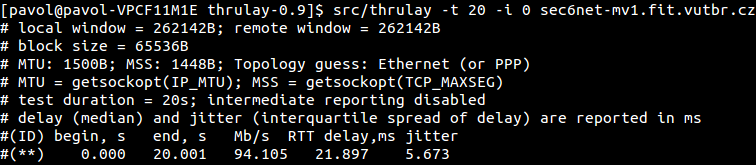
\includegraphics{img/thrulay_tcp.png}}
                   \caption{Ukážka spustenia nástroja Thrulay pre meranie TCP 
                    priepustnosti.}
               \label{thrulay_tcp}
           \end{center}
       \end{figure}

\newpage

       Ďalší test na obrázku \ref{thrulay_udp}
       ukazuje meranie pomocou transportného protokolu UDP. Výsledok
       tohto merania nám poskytuje informácie o~oneskorení a~jeho rozptylu,
       ďalej strate, duplikácii a~zmene poradia paketov. Posledné 
       dva parametre boli pri základnom meraní vždy nulové. V~ďalšej
       kapitole zameranej na merania zistíme, či sa výsledky zmenia.

       \begin{figure}[H]
           \begin{center}
                   \scalebox{0.65}{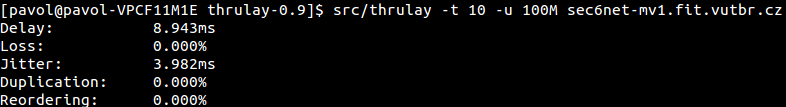
\includegraphics{img/thrulay_udp.png}}
                   \caption{Ukážka spustenia nástroja Thrulay pre meranie
                   pomocou protokolu UDP.}
               \label{thrulay_udp}
           \end{center}
       \end{figure}

        \subsection{Nekorektné správanie} \label{thrulay_chyby}
        Neschopnosť naviazať spojenie pomocou sieťového protokolu IPv6.

        \subsection{Zhodnotenie} \label{thrulay_zhod}
        Nástroj hodnotíme veľmi kladne pre jeho jednoduché ovládanie
        a~inštaláciu, ktorá nevyžaduje ďalšie podporné aplikácie.
        Sklamala nás neschopnosť testovania priepustnosti pod protokolom
        UDP. Testovanie pod protokolom UDP sa 
        zameriava na zistenie jednosmerného oneskorenia pri vyťaženosti linky 
        na danej priepustnosti. Toto meranie oneskorenia môže byť zavádzajúce,
        pretože v~niektorých meraniach sme dostali záporné hodnoty, čo môže byť
        spôsobené rozdielnym časom na koncových staniciach. Preto nedoporučujeme
        testovanie oneskorenia pomocou tohto nástroja.
        Tabuľky \ref{tab_thrulay_param} a~\ref{tab_thrulay_vlast} poskytujú
        informácie o~možnostiach testovania tohto nástroja.

        \begin{table}[H]
            \begin{center}
                \begin{tabular}{|c|c|c|c|c|c|}
                    \hline
                    \textbf{TCP priep.}  &  \textbf{UDP priep.}  &
                    \textbf{Oneskorenie} & \textbf{Jitter} &
                    \textbf{Zmena poradia} & \textbf{Strata} \\
                    \hline
                    $\surd$ & & & & $\surd$ & $\surd$\\ 
                    \hline
                \end{tabular}
                \caption{Merateľné parametre siete pomocou nástroja Thrulay.}
                \label{tab_thrulay_param}
            \end{center}
        \end{table}

        \begin{table}[H]
            \begin{center}
                \begin{tabular}{|c|c|c|c|c|}
                    \hline
                    \textbf{Linux}  &  \textbf{Windows}  &
                    \textbf{FreeBSD} & \textbf{IPv6} &
                    \textbf{NAT} \\
                    \hline
                    $\surd$ &  & $\surd$ &  & $\surd$ \\ 
                    \hline
                \end{tabular}
                \caption{Ďalšie vlastnosti nástroja Thrulay.}
                \label{tab_thrulay_vlast}
            \end{center}
        \end{table}

    \section{Nástroj Nuttcp}
        V~80. rokoch 20. storočia so~vznikom protokolu TCP bol implementovaný 
        nástroj Ttcp pre meranie jeho priepustnosti. Ttcp bol vtedy zaradený 
        medzi štandardné utility systému BSD. Od tej doby vzniklo viacero
        projektov, ktoré sú založené na tomto pôvodnom nástroji. Medzi jeho
        známe rozšírenia patrí Nttcp, v~ktorom sú implementované rozširujúce
        možnosti testovania. Z~Nttcp vychádza nástroj Nuttcp, ktorému sa budeme
        podrobnejšie venovať. Z~jeho predchodcov si zachoval vlastnosti ako
        jednoduchosť ovládania a~implementáciu v~jednom 
        zdrojovom texte. Pre výber tohto nástroja sme sa rozhodli, pretože je
        v~súčasnej dobe stále vyvíjaný a~poskytuje najlepšie možnosti
        testovania. Taktiež sa nachádza v~mnohých balíčkových repozitároch 
        distribúcie Linuxu.

        Nuttcp je nástroj vyvinutý na meranie TCP a~UDP priepustnosti. 
        Autori ho priamo porovnávajú s~riešením
        Iperf. Podľa ich názoru je to najlepší dostupný nástroj 
        pre svoju jednoduchosť, ľahkosť použitia a~schopnosti merania
        \cite{nuttcp_home}. Skladá sa z~jedného spustiteľného súboru, ktorý
        implementuje klienta a~démona súčasne. Pre účely testovania bola
        vybratá verzia 7.2.1
        \footnote{Dostupná na \url{http://lcp.nrl.navy.mil/nuttcp/}}.

        \subsection{Architektúra}\label{nuttcp_arch}
        Taktiež sa jedná o~aplikáciu typu klient\,--\,server. Obe
        strany sú implementované v~jednom spustiteľnom súbore. Použitím 
        prepínača sa vyberie zvolená strana. Komunikácia prebieha
        na dvoch portoch, z~nich jeden je komunikačný (5000) a~druhý
        určený na prenos testovaných dát (5001).

        \subsection{Softvérové nároky} \label{nuttcp_sw}
        Nuttcp pre svoju činnosť nepotrebuje žiadne doplnkové aplikácie,
        napríklad kvôli synchronizácii času. Medzi podporované systémy 
        patrí Linux, FreeBSD, Solaris a~Windows. Nástroj môžeme nájsť vo
        väčšine balíčkových repozitárov. Výhodná je kompilácia zo zdrojových
        textov, pretože sa nástroj stále vyvíja. Pre úspešnú kompiláciu je 
        potrebný prekladač jazyka C a~knižnica glibc.
        Nasledujúca ukážka demonštruje jeden z~príkladov kompilácie.

        \begin{flushleft}
            \texttt{\$ cc -O3 -o nuttcp  nuttcp-7.2.1.c} \\
        \end{flushleft}

        \subsection{Popis vybraných parametrov} \label{nuttcp_param}
        Tabuľka \ref{tab_nuttcp_parametre} poskytuje výpis najdôležitejších
        prepínačov. Aj napriek tomu, že je klient a~server implementovaný
        v~jednom spustiteľnom súbore, prepínače sme rozdelili do dvoch skupín
        na ovládanie klienta a~démona.

        \begin{table}[H]
            \begin{center}
                \begin{tabular}{|l|p{11cm}|}
                    \hline
                     \textbf{Parameter}  &  \textbf{Popis}  \\
                    \hline  
                    \multicolumn{2}{|c|}{Spoločné prepínače} \\
                    \hline
                    -p \textless číslo\textgreater & číslo portu\\
                    -v & doplnkové výpisy\\
                    -4 & použitie IPv4\\
                    -6 & použitie IPv6\\
                    \hline
                    \multicolumn{2}{|c|}{Prepínače pre klienta} \\
                    \hline
                    -r & prevedie testovanie od servera ku klientovi\\
                    -u  & použitie protokolu UDP, testuje 
                        priepustnoť do 1 Mbps \\
                    -R \textless číslo\textgreater[MG]& určí maximálnu 
                        testovanú priepustnosť \\
                    -T  \textless číslo\textgreater[mh]& dĺžka trvania testu,
                        m\,--\,minúty, h\,--\,hodiny, bez značky sekundy\\
                    -i \textless číslo\textgreater & časový interval výpisov
                        merania \\
                    \hline  
                    \multicolumn{2}{|c|}{Prepínače pre démona} \\
                    \hline
                    -S &  spustí démona\\ 
                    --nofork &  program sa spustí na popredí\\
                    \hline
                \end{tabular}
                \caption{Vybrané parametre nástroja Nuttcp.} 
                \label{tab_nuttcp_parametre}
            \end{center}
        \end{table}

        \noindent Pre správne spustenie klienta stačí zadať jeden argument: IP adresu
        alebo doménové meno stanice kde je spustená serverová časť. Niekedy je
        nutné pre nadviazanie spojenia použiť prepínač určujúci sieťový
        protokol. Druhý príkaz spustí démona na popredí.

        \begin{flushleft}
            \texttt{\$ nuttcp <adresa>} \\
            \texttt{\$ nuttcp -S --nofork}
        \end{flushleft}

       \subsection{Ukážka testov} \label{nuttcp_testy}
        Prvý test na obrázku \ref{nuttcp_tcp} obsahuje výsledok z~merania
        TCP priepustnosti. Poskytuje informácie o~veľkosti prenesených 
        dát za časovú jednotku a~dosiahnutú priepustnosť. Výpis obsahuje taktiež
        informácie o~RTT v~milisekundách a~vyťaženie CPU lokálnej (TX)
        a~koncovej (RX) stanice. Taktiež údaj o~znovu poslaných paketoch.
        Vypísaná hodnota RTT je v~porovnaní s~aplikáciou Ping
        veľmi podobná, preto ju môžeme považovať za správnu. Test sa implicitne 
        spustí na 10 sekúnd. Toto chovanie môžeme zmeniť použitím prepínača
        \texttt{-T} viď \ref{tab_nuttcp_parametre}.

       \begin{figure}[H]
           \begin{center}
                   \scalebox{0.65}{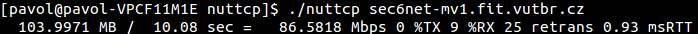
\includegraphics{img/nuttcp_tcp.png}}
                   \caption{Ukážka spustenia nástroja Nuttcp pre meranie TCP
                   priepustnosti.}
               \label{nuttcp_tcp}
           \end{center}
       \end{figure}
        
       Nasledujúci obrázok \ref{nuttcp_udp} demonštruje výpis nástroja pre
       meranie UDP priepustnosti. Pri spustení bol použitý parameter, ktorý
       spôsobil použitie UDP protokolu a~špecifikovanie maximálnej 
       testovanej priepustnosti, ktorá bola v~tomto prípade 100 Mbps.
       Oproti výstupu z~merania TCP priepustnosti
       obsahuje informácie o~celkovom počte poslaných a~zahodených paketov. 
       Z~toho je vypočítaná stratovosť paketov.

       \begin{figure}[H]
           \begin{center}
                   \scalebox{0.65}{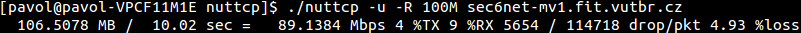
\includegraphics{img/nuttcp_udp.png}}
                   \caption{Ukážka spustenia nástroja Nuttcp pre meranie UDP
                   priepustnosti.}
               \label{nuttcp_udp}
           \end{center}
       \end{figure}

        \subsection{Nekorektné správanie} \label{nuttcp_chyby}
        Neschopnosť spustiť testovanie pod protokolom IPv6.
        Klientská časť aplikácie niekedy nebola schopná nadviazať spojenie. Túto
        chybu je možné potlačiť použitím prepínača \texttt{-4}, ktorý vynúti
        použitie sieťového protokolu IPv4.

        \subsection{Zhodnotenie} \label{nuttcp_zhod}
        Hlavnou prednosťou tohto nástroja je jednoduchosť vo všetkých smeroch.
        Je implementovaný v~jedinom súbore so~zdrojovým textom, čo uľahčuje
        a~urýchľuje
        kompiláciu. Užívateľské rozhranie v~podobe prepínačov je tiež veľmi 
        intuitívne a~jednoduché.  Výpisy sú zrozumiteľné a~poskytujú
        len tie najdôležitejšie informácie. Aj keď nástroj nedokáže odmerať
        oneskorenie a~jeho rozptyl, poskytuje základnú funkcionalitu pre meranie 
        priepustnosti.

        Pri testovaní UDP priepustnosti klientská časť vyťažovala CPU na
        maximum. Toto správanie považujeme za nedostatok implementácie.

        \begin{table}[H]
            \begin{center}
                \begin{tabular}{|c|c|c|c|c|c|}
                    \hline
                    \textbf{TCP priep.}  &  \textbf{UDP priep.}  &
                    \textbf{Oneskorenie} & \textbf{Jitter} &
                    \textbf{Zmena poradia} & \textbf{Strata} \\
                    \hline
                    $\surd$ & $\surd$ & & & & $\surd$\\ 
                    \hline
                \end{tabular}
                \caption{Merateľné parametre siete pomocou nástroja Nuttcp.}
                \label{tab_nuttcp_param}
            \end{center}
        \end{table}

        \begin{table}[H]
            \begin{center}
                \begin{tabular}{|c|c|c|c|c|}
                    \hline
                    \textbf{Linux}  &  \textbf{Windows}  &
                    \textbf{FreeBSD} & \textbf{IPv6} &
                    \textbf{NAT} \\
                    \hline
                    $\surd$ & $\surd$ & $\surd$ &  & $\surd$ \\ 
                    \hline
                \end{tabular}
                \caption{Ďalšie vlastnosti nástroja Nuttcp.}
                \label{tab_nuttcp_vlast}
            \end{center}
        \end{table}

    \section{Nástroj BWPing}
        Tento nástroj sme vybrali do našej práce pre jeho jedinečnosť
        implementácie testovania. Slúži na meranie priepustnosti 
        a~času RTT. Testovanie prebieha pomocou protokolu ICMP. Program posiela
        správy ICMP Echo Request a~čaká na doručenie Echo Replay
        \cite{bwping_home}. Týmto
        mechanizmom zisťovania priepustnosti sa líši od všetkých klasických
        nástrojov. Je to excelentné riešenie, ktoré nepotrebuje druhú koncovú
        stanicu so spusteným procesom tejto aplikácie.
        Táto implementácia má však svoje nedostatky. Ak sú po ceste filtrované ICMP
        správy, tento mechanizmus nefunguje. Meranie môže ovplyvniť taktiež
        aplikovaná QoS na meranej linke.
        Pre účely testovania bola vybratá verzia 1.7
        \footnote{Dostupná na \url{http://bwping.sourceforge.net/index.php}}.

        \subsection{Architektúra}\label{bwping_arch}
        Kvôli implementácii merania pomocou správ ICMP táto konzolová aplikácia 
        vyžaduje iba klientskú časť. Aplikácia bola rozdelená do dvoch
        spustiteľných súborov, ktoré sa líšia použitím sieťového protokolu IPv4
        a~IPv6. Pre IPv4 je vyčlenený \texttt{bwping} a~pre IPv6
        \texttt{bwping6}. Je implementovaný v~jazyku C s~použitím BSD soketov
        typu RAW.

        \subsection{Softvérové nároky} \label{bwping_sw}
        Nástroj je dostupný v~zdrojových textoch, takže je potrebná priama 
        kompilácia. Pre túto činnosť je potrebný prekladač jazyka C a~knižnica
        glibc. Dôležité je poznamenať, že pre spustenie musíme mať práva super
        užívateľa kvôli práci so soketmi typu RAW. 

\newpage

        \subsection{Popis vybraných parametrov} \label{bwping_param}
        Pre základné spustenie nástroj potrebuje tri povinné prepínače: prenosovú
        rýchlosť, veľkosť paketu a~celkový objem prenesených dát. Tabuľka 
        \ref{tab_bwping_parametre} obsahuje výpis prepínačov.

        \begin{table}[H]
            \begin{center}
                \begin{tabular}{|l|p{11cm}|}
                    \hline
                     \textbf{Parameter}  &  \textbf{Popis}  \\
                    \hline
                    -b \textless číslo\textgreater & prenosová rýchlosť v~kbps\\
                    -s \textless číslo\textgreater & veľkosť paketu v~bajtoch\\
                    -v \textless číslo\textgreater & objem poslaných dát
                        v~bajtoch\\
                    -r \textless číslo\textgreater & interval výpisov 
                        (implicitne vypnuté) \\
                    -B \textless adresa\textgreater & nastaví adresu
                        odchádzajúcich paketov\\
                    \hline
                \end{tabular}
                \caption{Vybrané parametre nástroja BWPing.} 
                \label{tab_bwping_parametre}
            \end{center}
        \end{table}

        \noindent Nasledujúca ukážka demonštruje spustenie nástroja. Pre spustenie sú 
        všetky parametre povinné.

        \begin{flushleft}
            \texttt{\$ bwping -b <číslo> -s <číslo> -v <číslo> <adresa>} 
        \end{flushleft}

        \subsection{Ukážka testov} \label{bwping_testy}
        Na nasledujúcej ukážke si uvedieme spustenie s~výstupom merania. Keďže
        pracuje so správami ICMP, nie je možné vybrať transportný protokol.
        Testovala sa maximálna priepustnosť 90 Mbps s~ICMP paketmi o~veľkosti 61 KB
        a~celkové množstvo poslaných dát bolo 9 MB. Výstup nám poskytuje
        informácie o~počte poslaných a~prijatých paketov, dosiahnutej
        priepustnosti a~čase RTT, ktorý bol nameraný pri dosiahnutí nameranej
        priepustnosti.

       \begin{figure}[H]
           \begin{center}
                   \scalebox{0.50}{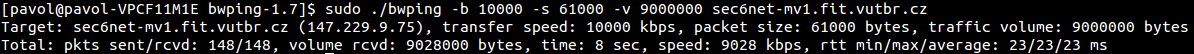
\includegraphics{img/bwping.png}}
                   \caption{Ukážka spustenia nástroja BWPing.}
               \label{bwping}
           \end{center}
       \end{figure}
       
        \subsection{Nekorektné správanie} \label{bwping_chyby}
        Implementačné chyby tohto nástroja neboli zaznamenané,
        jedná sa o~jednoduchú utilitu, ktorá je dobre odladená. 
        Ak pri testovaní nastavíme príliš veľké hodnoty prepínačov, 
        vypíše hlášku 
        \texttt{bwping: sendto() failed: No buffer space available}.
        Toto je jediné zistené nekorektné správanie, ktoré môže 
        znepríjemňovať testovanie.

        \subsection{Zhodnotenie} \label{bwping_zhod}
        Prednosťou tohto nástroja je, že nepotrebuje pre svoju činnosť serverovú
        časť. Týmto spôsobom sme schopní odmerať priepustnosť voči ľubovoľnej
        stanici, na ktorú nemáme prístup. 

        Nevýhodou je použitie protokolu ICMP. Mnohí poskytovatelia pripojenia
        tieto správy filtrujú, tak nie je možné úspešne testovanie. Taktiež
        podpora kvality služieb môže ovplyvňovať výsledky. Hodnoty nameranej 
        priepustnosti nikdy nezodpovedali reálne dostupnej. Taktiež uvedené
        problémy s~ICMP protokolom znižujú jeho použiteľnosť. 
        
        Nástroj
        odporúčame len na experimentálne účely, alebo použitie vo~vlastnej sieti 
        na overenie konektivity. Tabuľky \ref{tab_bwping_param}
        a~\ref{tab_bwping_vlast} obsahujú súhrn možností testovania s~týmto
        nástrojom. Nameranú priepustnosť týmto nástrojom sme označili, že patrí
        pod protokol UDP.

        \begin{table}[H]
            \begin{center}
                \begin{tabular}{|c|c|c|c|c|c|}
                    \hline
                    \textbf{TCP priep.}  &  \textbf{UDP priep.}  &
                    \textbf{Oneskorenie} & \textbf{Jitter} &
                    \textbf{Zmena poradia} & \textbf{Strata} \\
                    \hline
                     & $\surd$ & & & & $\surd$\\ 
                    \hline
                \end{tabular}
                \caption{Merateľné parametre siete pomocou nástroja BWPing.}
                \label{tab_bwping_param}
            \end{center}
        \end{table}

        \begin{table}[H]
            \begin{center}
                \begin{tabular}{|c|c|c|c|c|}
                    \hline
                    \textbf{Linux}  &  \textbf{Windows}  &
                    \textbf{FreeBSD} & \textbf{IPv6} &
                    \textbf{NAT} \\
                    \hline
                    $\surd$ &  & $\surd$ &  $\surd$ & $\surd$ \\ 
                    \hline
                \end{tabular}
                \caption{Ďalšie vlastnosti nástroja BWPing.}
                \label{tab_bwping_vlast}
            \end{center}
        \end{table}

    \section{Celkové vyhodnotenie} \label{nastroje_zhod}
    Po podrobnom otestovaní vybratých open source nástrojov, ktoré tvoria 
    väčšinu dostupných aplikácii s~týmto zameraním, je nutné ich medzi sebou
    porovnať. Každý z~nástrojov je špecifický a~ponúka rôzne možnosti
    testovania. Tabuľka \ref{tab_zhod_param} obsahuje informácie o~možnosti
    použitia jednotlivých utilít na meranie špecifických parametrov sieťového 
    prenosu, ktoré sme vybrali v~kapitole \ref{metodika_parametre}. Naša
    metodika pre hodnotenie nástrojov skúma aj iné vlastnosti nástrojov. 
    Tabuľka \ref{tab_zhod_vlast} obsahuje tieto funkcionálne vlastnosti uvedené v~kapitole 
    \ref{metodika_vlastnosti}. Medzi vlastnosti sme pridali fakt, či je nástroj 
    aktívne vyvíjaný. Ak bola posledná verzia vydaná v~roku 2012, vývoj pokračuje. 

    Z~výsledkov z~tabuľky \ref{tab_zhod_param} je zrejmé, že každá utilita
    poskytuje iné možnosti testovania. Väčšina dokáže odmerať TCP alebo UDP
    priepustnosť. 
    Nástroje, ktoré umožňujú testovanie pod transportným protokolom UDP,
    využívajú jeho vlastnosti a~dokážu odmerať stratovosť, zmenu poradia 
    a~rozptyl oneskorenia paketov.

    Testovania jednosmerného oneskorenia medzi dvoma stanicami je
    možné len v~prípade, ak majú dostatočne synchronizovaný čas. Inak sú
    výsledky nepresné. Tento parameter dokáže odmerať OWAMP a~Thrulay. Avšak
    Thrulay nevyžaduje synchronizáciu času, takže ho do tejto skupiny
    neradíme. Ostatné nástroje, ktoré nie sú schopné odmerať jednosmerné
    oneskorenie, poskytujú údaj o~RTT pri nameranej priepustnosti.
    
    Nástroj BWCTL sme do súhrnných tabuliek neuvádzali, pretože pre účely
    testovania používa Iperf, Nuttcp a~Thrulay. Ak by sme schopnosti týchto
    troch nástrojov spojili, dokázali by odmerať takmer všetky parametre sieťového 
    prenosu, ktoré sledujeme. Zložitosť testovania s~týmto nástrojom je kvôli
    synchronizácii času a~zdĺhavej inštalácii vysoká. Pre naše účely je BWCTL
    nevhodný nástroj.
    
    \begin{table}[h!]
        \begin{center}
            \begin{tabular}{|m{1.5cm}|m{1.4cm}|m{1.4cm}|m{2.6cm}|m{1.2cm}|m{1.7cm}|m{1.4cm}|}
                \hline
                 \textbf{Nástroj}  &  \textbf{TCP priep.} &
                 \textbf{UDP priep.} & \textbf{Oneskorenie} &
                 \textbf{Jitter} &
                 \textbf{Zmena poradia} & 
                 \textbf{Strata}\\ 
                \hline
                Iperf &\multicolumn{1}{c|}{$\surd$}&
                    \multicolumn{1}{c|}{$\surd$}&\multicolumn{1}{c|}{}&
                    \multicolumn{1}{c|}{$\surd$}&\multicolumn{1}{c|}{} &
                    \multicolumn{1}{c|}{$\surd$} \\
                Netperf &\multicolumn{1}{c|}{$\surd$}&
                    \multicolumn{1}{c|}{}&\multicolumn{1}{c|}{}&
                    \multicolumn{1}{c|}{}&\multicolumn{1}{c|}{} &
                    \multicolumn{1}{c|}{} \\
                OWAMP &\multicolumn{1}{c|}{}&
                    \multicolumn{1}{c|}{}&\multicolumn{1}{c|}{$\surd$}&
                    \multicolumn{1}{c|}{$\surd$}&\multicolumn{1}{c|}{$\surd$} &
                    \multicolumn{1}{c|}{$\surd$} \\
                Thrulay &\multicolumn{1}{c|}{$\surd$}&
                    \multicolumn{1}{c|}{}&\multicolumn{1}{c|}{}&
                    \multicolumn{1}{c|}{}&\multicolumn{1}{c|}{$\surd$} &
                    \multicolumn{1}{c|}{$\surd$} \\
                Nuttcp &\multicolumn{1}{c|}{$\surd$}&
                    \multicolumn{1}{c|}{$\surd$}&\multicolumn{1}{c|}{}&
                    \multicolumn{1}{c|}{}&\multicolumn{1}{c|}{} &
                    \multicolumn{1}{c|}{$\surd$} \\
                BWPing &\multicolumn{1}{c|}{}&
                    \multicolumn{1}{c|}{$\surd$}&\multicolumn{1}{c|}{}&
                    \multicolumn{1}{c|}{}&\multicolumn{1}{c|}{} &
                    \multicolumn{1}{c|}{$\surd$} \\
                    \hline
            \end{tabular}
            \caption{Možnosti nástrojov testovať parametre sieťového prenosu.} 
            \label{tab_zhod_param}
        \end{center}
    \end{table}

\newpage 

    Všetky testované nástroje sú určené pre unixové operačné systémy.
    Podpora Windows je zabezpečené
    prostredníctvom Cygwin\footnote{Dostupné na \url{http://www.cygwin.com/}}.
    Utility, ktoré sú prispôsobené na Windows, je možné
    stiahnuť preložené v~binárnej forme. 
    
    Ako je vidieť z~tabuľky
    \ref{tab_zhod_vlast}, všetky aplikácie okrem OWAMP správne fungujú s~prekladom adries. 
    Podpora IPv6 bola uvedená v~manuáloch u~všetkých nástrojov. Reálne 
    testovanie ukázalo skutočnú funkcionalitu. Projekty všetkých uvedených
    nástrojov aktívne pokračujú, čo je dôležité pre budúce využite.

    \begin{table}[h!]
        \begin{center}
            \begin{tabular}{|c|c|c|c|c|c|c|}
                \hline
                \textbf{Nástroj}  &  \textbf{Linux} & \textbf{Windows} &
                \textbf{FreeBSD} & \textbf{IPv6} &  \textbf{NAT} &
                \textbf{Aktívny vývoj}\\ 
                \hline
                Iperf & $\surd$ & $\surd$ &  & $\surd$ & $\surd$ & $\surd$\\
                Netperf & $\surd$ & $\surd$ & $\surd$ &  & $\surd$ & $\surd$\\
                OWAMP & $\surd$ &  & $\surd$ & $\surd$ & & $\surd$\\
                Thrulay & $\surd$ &  & $\surd$ & $\surd$ & $\surd$ & $\surd$\\
                Nuttcp & $\surd$ & $\surd$ & $\surd$ &  & $\surd$ & $\surd$ \\
                BWPing & $\surd$ & & $\surd$ & $\surd$ & $\surd$ & $\surd$\\
                \hline
            \end{tabular}
            \caption{Ďalšie vlastnosti testovaných nástrojov.} 
            \label{tab_zhod_vlast}
        \end{center}
    \end{table}

    Výsledky tejto kapitoly nám pomohli zistiť, ktoré parametre sieťového
    prenosu sa dajú odmerať jednotlivými nástrojmi. V~ďalšej kapitole vytvoríme
    metodiku, pomocou ktorej utility otestujeme na reálnej sieti. Z~tabuľky
    \ref{tab_zhod_param} vyberieme parametre sieťového prenosu, ktoré budeme
    na reálnej sieti testovať.

\chapter{Testovanie na reálnej sieti} \label{testovanie}
Po preskúmaní nástrojov sme ich boli schopní medzi sebou
porovnať na  úrovni funkcionality.
Ďalším krokom tejto práce je testovanie na reálnej sieti. Následná
analýza výsledkov meraní nám umožní vyhodnotiť použiteľnosť nástrojov s~ohľadom na 
správnosť výsledkov. Cieľom tejto kapitoly bude určiť nástroj vhodný
na meranie vybraného parametra sieťového prenosu. 

Prvý krok spočíva vo vytvorení metodiky testovania. Tejto téme sa venuje
kapitola \ref{test_metodika}. Keďže výsledky merania budú v~číselnej podobe
a~testovanie ovplyvňuje veľké množstvo nezávislých faktorov, je nutné merania
uskutočniť opakovane. Tomuto problému sa venuje kapitola \ref{test_stat}. 
Po zhotovení metodiky a~štatistickej úprave výsledkov budeme schopní výsledky
vyhodnotiť v~kapitole \ref{test_vys}.

    \section{Metodika testovania} \label{test_metodika}
    Metodika testovania nástrojov na reálnej sieti musí zahŕňať viacero 
    faktorov. V~prvok kroku je potrebné vyčleniť parametre sieťového prenosu, 
    ktoré budeme merať. Keďže nástroje poskytujú rozličné testovacie možnosti,
    parametre je nutné vybrať tak, aby boli merateľné väčšinou nástrojov. 
    Z~tabuľky \ref{tab_zhod_param} môžeme vidieť, že tu patrí
    priepustnosť oboch transportných protokolov a~strata paketov. 
    K~týmto vlastnostiam pridáme jednosmerné oneskorenie, pretože meranie tohto 
    parametra poskytuje iba nástroj OWAMP. Získaná hodnota nás bude zaujímať
    s~porovnaním s~hodnotou RTT získanou pomocou utility Ping. 
    Ďalej je nutné zaistiť, aby testovanie každého nástroja bolo rovnaké.
    Tým myslíme dĺžku trvania testu a~čas, v~ktorom bol spustený. Kvôli rôznej
    vyťaženosti liniek internetu v~čase.

    \noindent Parametre sieťového prenosu, ktoré budeme merať:
    \begin{itemize}
        \item TCP priepustnosť.
        \item UDP priepustnosť.
        \item Strata paketov.
        \item Jednosmerné oneskorenie.
    \end{itemize}

\newpage

    \subsection{Vstupné podmienky} \label{test_podmienky}
        Keďže testovanie neprebieha v~laboratórnych podmienkach, ale na reálnej
        sieti cez internet, rôzne dátové toky môžu ovplyvňovať namerané hodnoty.
        V~neposlednom rade merania môžu ovplyvniť aj iné procesy bežiace na
        koncových staniciach, obsluhe hardvérových prerušení a~podobné príčiny.
        Preto budeme merania robiť v~priebehu celého dňa s~rozostupom 6 hodín. 
        Takto uskutočníme celkovo 4 merania za 24 hodín. Prvé zahájime v~čase 00:00.
        
        Na koncových staniciach, medzi ktorými prebiehalo testovanie, budú
        povolené len základné služby, aby testovanie bolo čo najmenej ovplyvnené 
        inými procesmi. Server, na ktorom budú spustené procesy démonov, má
        operačný systém Red Hat Enterprise Linux Server 6.3 (Santiago). Stanica,
        z~ktorej budú spúšťané klientské časti utilít, disponuje operačným
        systémom Ubuntu 12.10. 

    \subsection{Rozmiestnenie} \label{test_rozmiestnenie}
        Testovanie bude prebiehať vždy voči stanici s~adresou 
        sec6net-mv1.fit.vutbr.cz s~gigabitovým pripojením do internetu. 
        Tento školský server je umiestnený v~Brne. Stanica, z~ktorej
        bude spúšťané meranie prostredníctvom klientských častí nástrojov, má sieťovú
        kartu s~maximálnou prenosovou rýchlosťou 100 Mbps.
        Na obrázku \ref{internet} je znázornené rozmiestnenie všetkých testovacích 
        staníc. Väčšina koncových klientských staníc sa nachádza za prekladom adries.
        Preto neuvádzame ich IP adresy. 

        Meranie voči serveru v~Brne bolo robené z~troch lokalít
        s~rôznym pripojením k~internetu. Myslíme tým maximálnu priepustnosť uvedenú
        v~zmluve s~ISP. Prvá lokalita je Brno, kde máme k~dispozícii pripojenie
        s~rýchlosťou 100 Mbps. Počet skokov v~dobe testovania bol 7. Ďalšia stanica 
        je umiestnená na Slovensku s~pripojením 3 Mbps. Počet skokov k~serveru
        v~Brne bol 11. Posledné meranie prebiehalo zo Švajčiarska. Tam sme mali
        internetové pripojenie s~maximálnou rýchlosťou 5 Mbps. V~zmluve
        s~poskytovateľom internetového pripojenia je špecifikovaná maximálna
        priepustnosť. Provider však v~zmluve uvádza, že priepustnosť môže
        dosahovať aj veľmi nízke hodnoty, podľa lokality prípojky, pretože
        pripojenie je poskytované v~rámci celej siete \emph{Swisscom
        \footnote{Hlavný telekomunikačný provider v~Švajčiarsku}}.
        Počet skokov v~dobe testovania bol 13. Tabuľka \ref{net_parametre}
        obsahuje informácie o~parametroch internetových pripojení koncových
        bodov a~počet skokov k~serveru v~Brne.

       \begin{figure}[H]
           \begin{center}
                   \scalebox{0.58}{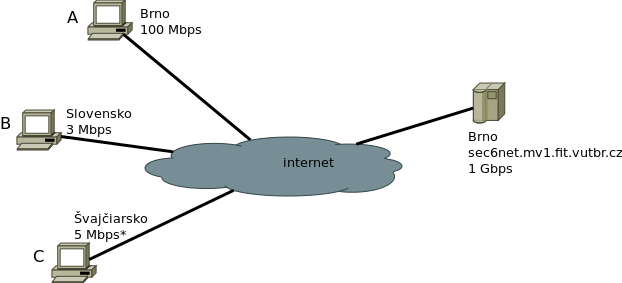
\includegraphics{img/internet.png}}
                   \caption{Náčrt testovanej topológie.}
               \label{internet}
           \end{center}
       \end{figure}

        \begin{table}[h!]
            \begin{center}
                \begin{tabular}{|c|c|c|}
                    \hline
                    Miesto & Priepustnosť uvedená v~SLA [Mbps] & Počet skokov\\  
                    \hline
                    Brno        & 100 & 7 \\
                    \hline
                    Slovensko   & 3   & 11 \\
                    \hline
                    Švajčiarsko & 5   & 13 \\
                    \hline
                \end{tabular}
                \caption{Parametre internetového pripojenia koncových bodov.} 
                \label{net_parametre}
            \end{center}
        \end{table}

     \subsection{Testy} \label{test_testy}
        V~jednotlivých podkapitolách budú uvedené podrobnejšie informácie
        o~zvolených testoch. Pre každý test je uvedený cieľ, nastavenie v~podobe 
        dĺžky trvania alebo počte odoslaných paketov a~jednotky, v~ktorých budú
        uvedené výsledky. Pre všetky testy okrem jednosmerného oneskorenia, viď
        \ref{metod_jednos_ones}, platia podmienky uvedené
        v~\ref{test_podmienky} a~rozmiestnenie v~\ref{test_rozmiestnenie}. 

        \subsubsection{Meranie TCP a~UDP priepustnosti}
        Cieľom tohto testovania je odmerať najväčšiu možnú priepustnosť medzi
        koncovými stanicami. Priepustnosť bude meraná pod transportným
        protokolom UDP a~TCP. Dĺžka testu bude nastavená na 20 sekúnd. 
        
        Pri
        testovaní maximálnej UDP priepustnosti je potrebné špecifikovať
        maximálnu priepustnosť. V~tabuľke \ref{udp_max_throu} sú uvedené
        hodnoty, ktoré boli použité pre špecifikovanie maximálnej UDP
        priepustnosti. Testovaná priepustnosť pre Švajčiarsko je oproti zmluve
        s~ISP (maximálne 5 Mbps) menšia o~viac než polovicu. Ako je uvedené
        v~kapitole \ref{test_rozmiestnenie}, maximálna priepustnosť pripojenia
        závisí od umiestnenia prípojky. V~našom prípade pripojenie bolo v~dobe 
        merania pomalšie než 1 Mbps. Preto sme zvolili uvedenú hodnotu 2 Mbps.
        Ak zvolíme príliš veľké číslo, výstup
        nástrojov bude signalizovať veľké percento stratovosti paketov.
        Výsledná nameraná hodnota bude uvedená v~jednotkách Mbps.

        \begin{table}[h!]
            \begin{center}
                \begin{tabular}{|c|c|}
                    \hline
                    Miesto & Nastavená maximálna priepustnosť [Mbps] \\  
                    \hline
                    Brno        & 100,00  \\
                    \hline
                    Slovensko   & 3,50   \\
                    \hline
                    Švajčiarsko & 2,00 \\
                    \hline
                \end{tabular}
                \caption{Hodnoty nastavenej maximálnej priepustnosti pri meraní
                UDP priepustnosti.} 
                \label{udp_max_throu}
            \end{center}
        \end{table}
        
        Pre meranie TCP priepustnosti sme vybrali nástroje: Iperf, Netperf,
        Thrulay a~Nuttcp. Do testu UDP priepustnosti: Iperf, Nuttcp a~BWPing.

        \subsubsection{Strata paketov}
        Cieľom tohto testu bude určiť percento stratených paketov k~celkovému
        počtu prenesených pri dosiahnutej maximálnej priepustnosti.
        Stratu paketov je možné merať len pod transportným protokolom UDP. 
        Nameraná
        hodnota bude uvedená v~percentách podľa vzťahu \ref{rovnica_strata}.
        Hodnoty prevzaté z~testovania UDP
        priepustnosti. Takto budeme schopní analyzovať stratovosť pri dosiahnutej
        maximálnej priepustnosti.

        \begin{eqnarray} \label{rovnica_strata}
            \frac{\text{stratené pakety}}{\text{celkový počet paketov}} * 100\ [\%]
        \end{eqnarray}
        
        Pre meranie straty paketov boli zahrnuté nástroje: Iperf, Nuttcp
a~Thrulay. BWPing sme nezahrnuli, pretože za stratu paketu počíta
        nedoručený paket ICMP Echo Reply k~odoslanému ICMP Echo Request.

        \subsubsection{Jednosmerné oneskorenie} \label{metod_jednos_ones}
        Cieľom tohto testu je určenie rozdielu jednosmerného oneskorenia 
        nameraného pomocou utility OWAMP a~polovičnej hodnoty RTT pomocou
        nástroja Ping. Týmto
        testom sa snažíme zistiť reálnu použiteľnosť nástroja OWAMP, pretože
        utilita Ping je dostupná vo všetkých bežne používaných systémoch.
        
        Pri meraní oneskorenia sme zvolili množstvo 50 testovacích paketov.
        Do výsledkov bude zahrnutá priemerná hodnota uvedená v~milisekundách.
        Keďže s~nástrojom OWAMP nie je možné testovať, ak sa klientská
        časť nachádza za prekladom adries, bude prevedené meranie 
        len z~miesta v~Brne, kde máme prístup k~verejnej IP adrese.

        \subsection{Štatistická úprava výsledkov} \label{test_stat}
        Výsledky získané pomocou testovaných utilít majú číselnú formu. Preto je
        možné ich upraviť a~získať informácie, ktoré nám bližšie pomôžu analyzovať 
        výsledky. Ako bolo uvedené v~\ref{test_podmienky}, test ovplyvňujú viaceré
        nezávislé faktory. Preto je nutné testovanie vykonať opakovane.

        Zo štatistického súboru získaných výsledkov z~nezávislých behov 
        spravíme aritmetický priemer podľa vzťahu \ref{rovnica_priemer}.
        Ďalšou významnou úpravou výsledkov 
        bude vypočítanie smerodajnej odchýlky, ktorá určuje, ako široko sú
        hodnoty rozložené v~množine viď \cite{statistika}. Tvar rovnice je
        uvedený v~\ref{rovnica_odchylka}.

        \begin{eqnarray} \label{rovnica_priemer}
            \overline{x} = \frac{1}{n} \sum_{i=0}^n x_{i}
        \end{eqnarray}
        \begin{eqnarray} \label{rovnica_odchylka}
            s~= \sqrt{\frac{1}{n} \sum_{i=1}^n (x_{i} - \overline{x})^2}
        \end{eqnarray}

    \section{Analýza výsledkov} \label{test_vys}
    Výsledky z~meraní sa nachádzajú v~príslušných podkapitolách. Každý test
    obsahuje tabuľku s~nameranými hodnotami a~stĺpcový graf, ktorý prehľadne
    znázorňuje výsledky. 

        \subsection{TCP Priepustnosť} \label{test_vys_tcp}
        Výsledky z~merania TCP priepustnosti sú uvedené v~tabuľkách
        \ref{tab_test_tcp} pre meranie z~Brna,
        \ref{tab_test_tcp_swiss} pre Švajčiarsko a~\ref{tab_test_tcp_sk} pre
        Slovensko. Pre
        prehľadnosť uvádzame tabuľku \ref{vys_tcp_priep}, v~ktorej sú údaje 
        o~priepustnosti uvedenej v~SLA a~nameranej. 
        
        Z~výsledkov môžeme zhodnotiť, že nameraná priepustnosť z~Brna
        a~Slovenska je približne rovnaká ako uvedená hodnota v~SLA. 
        Priemerná 
        priepustnosť zo Švajčiarska je 0.25 Mbps. Ako sme uviedli v~predošlých
        kapitolách, tamojší poskytovateľ pripojenia uviedol, že rýchlosť je 
        závislá na umiestnení prípojky. V~našom prípade sa prípojka nachádzala
        v~lokalite, 
        kde bola dostupná iba telekomunikačná sieť. Preto bola nameraná
        priepustnosť výrazne nižšia v~porovnaní s~hodnotou v~zmluve.
        
        Smerodajná odchýlka výsledkov jednotlivých nástrojov a~priemerne
        nameranej priepustnosti je pomerne malé číslo. V~prevedení na
        priepustnosť pre bod zo Slovenska je to 93 Kbps, čo je malá hodnota
        oproti priemernej 2940 Kbps. V~prepočte na percentá je to 3,16 \%
        z~nameranej priepustnosti.

        Po tejto analýze môžeme zhodnotiť, že výsledky meraní testovaných utilít
        sa odlišujú v~malej miere. Preto je nemožné priamo rozhodnúť, ktorý
        nástroj je na meranie TCP priepustnosti najlepší v~zmysle
        správnosti výsledkov. Pre meranie tohto parametra sieťového prenosu 
        odporúčame ľubovoľný z~testovaných nástrojov.

        \begin{table}[h!]
            \begin{center}
                \begin{tabular}{|c|m{4.3cm}|m{4cm}|m{3.4cm}|}
                    \hline
                    Miesto & Priemerná odmeraná TCP priepustnosť [Mbps] &
                    Smerodajná odchýlka nástrojov od priemeru &
                    Priepustnosť z~SLA [Mbps] \\  
                    \hline
                    Brno        &  \multicolumn{1}{c}{87,48} & 
                        \multicolumn{1}{|c|}{0,30} & \multicolumn{1}{c|}{100,00} \\
                    \hline
                    Slovensko   &  \multicolumn{1}{c}{2,94} & 
                        \multicolumn{1}{|c|}{0,093} & \multicolumn{1}{c|}{3,00} \\
                    \hline
                    Švajčiarsko &  \multicolumn{1}{c}{0,25} & 
                        \multicolumn{1}{|c|}{0,062} & \multicolumn{1}{c|}{5,00*}\\
                    \hline
                \end{tabular}
                \caption{Výsledky nameranej TCP priepustnosti.} 
                \label{vys_tcp_priep}
            \end{center}
        \end{table}

%TCP Brno
    \begin{table}[h!]
        \begin{center}
            \begin{tabular}{|c|c|c|c|c|}
                \hline
            Nástroj & Iperf [Mbps]& Netperf [Mbps]& Thrulay [Mbps]& Nuttcp [Mbps]\\ 
                \hline
                1.beh o~00:00 & 88,21 & 87,57 & 87,35 & 87,45 \\
                \hline
                2.beh o~06:00 & 87,76 & 87,39 & 87,21 & 87,10 \\
                \hline
                3.beh o~12:00 & 88,54 & 87,23 & 87,52 & 87,19 \\
                \hline
                4.beh o~18:00 & 87,25 & 87,13 & 87,95 & 86,74 \\
                \hline
                priemer & 87,94 & 87,33 & 87,51 & 87,12 \\
                \hline
                smerodajná odchýlka & \multicolumn{4}{c|}{0,30}\\
                \hline
            \end{tabular}
            \caption{Odmeraná TCP priepustnosť testovaných nástrojov z~Brna.} 
            \label{tab_test_tcp}
        \end{center}
    \end{table}
   \begin{figure}[H]
       \begin{center}
               \scalebox{0.67}{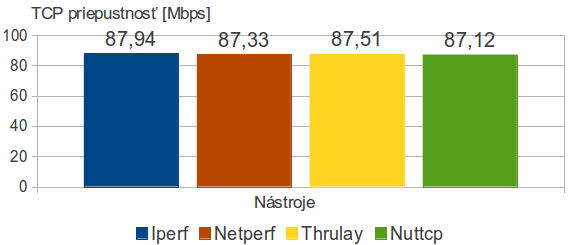
\includegraphics{img/cz_tcp.png}}
               \caption{Graf odmeranej TCP priepustnosti testovaných nástrojov
               z~Brna.}
           \label{tab_test_tcp_graf}
       \end{center}
   \end{figure}

%TCP SWISS
    \begin{table}[h!]
        \begin{center}
            \begin{tabular}{|c|c|c|c|c|}
                \hline
            Nástroj & Iperf [Mbps]& Netperf [Mbps]& Thrulay [Mbps]& Nuttcp [Mbps]\\ 
                \hline
                1.beh o~00:00 & 0,36 & 0,22 & 0,21 & 0,22 \\
                \hline
                2.beh o~06:00 & 0,36 & 0,22 & 0,21 & 0,22 \\
                \hline
                3.beh o~12:00 & 0,41 & 0,21 & 0,21 & 0,22 \\
                \hline
                4.beh o~18:00 & 0,37 & 0,22 & 0,21 & 0,22 \\
                \hline
                priemer       & 0,36 & 0,22 & 0,21 & 0,22 \\
                \hline
                smerodajná odchýlka & \multicolumn{4}{c|}{0,062}\\
                %√((1÷4)×((0.36−0.25)²+(0.22−0.25)²+(0.21−0.25)²+(0.22−0.25)²)
                \hline
            \end{tabular}
            \caption{Odmeraná TCP priepustnosť testovaných nástrojov zo
                Švajčiarska.} 
            \label{tab_test_tcp_swiss}
        \end{center}
    \end{table}
   \begin{figure}[H]
       \begin{center}
               \scalebox{0.67}{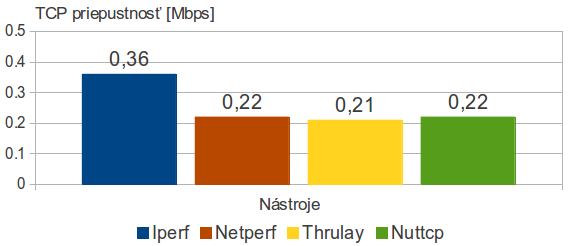
\includegraphics{img/swiss_tcp.png}}
               \caption{Graf odmeranej TCP priepustnosti testovaných nástrojov
               zo Švajčiarska.}
           \label{tab_test_tcp_swiss_graf}
       \end{center}
   \end{figure}

%TCP SK
    \begin{table}[h!]
        \begin{center}
            \begin{tabular}{|c|c|c|c|c|}
                \hline
            Nástroj & Iperf [Mbps]& Netperf [Mbps]& Thrulay [Mbps]& Nuttcp [Mbps]\\ 
                \hline
                1.beh o~00:00 & 3,10 & 2,86 & 2,91 & 2,89 \\
                \hline
                2.beh o~06:00 & 3,11 & 2,89 & 2,91 & 2,90 \\
                \hline
                3.beh o~12:00 & 3,12 & 2,83 & 2,86 & 2,87 \\
                \hline
                4.beh o~18:00 & 3,09 & 2,89 & 2,91 & 2,89 \\
                \hline
                priemer       & 3,10 & 2,87 & 2,90 & 2,89 \\
                \hline
                smerodajná odchýlka & \multicolumn{4}{c|}{0,093}\\
                \hline
            \end{tabular}
            \caption{Odmeraná TCP priepustnosť testovaných nástrojov zo
                Slovenska.} 
            \label{tab_test_tcp_sk}
        \end{center}
    \end{table}
   \begin{figure}[H]
       \begin{center}
               \scalebox{0.67}{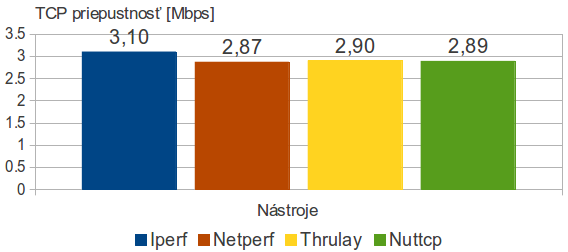
\includegraphics{img/sk_tcp.png}}
               \caption{Graf odmeranej TCP priepustnosti testovaných nástrojov
               zo Slovenska.}
           \label{tab_test_tcp_sk_graf}
       \end{center}
   \end{figure}

        \subsection{UDP Priepustnosť} \label{test_vys_udp}
        Výsledky z~merania UDP priepustnosti sa nachádzajú v~tabuľke
        \ref{tab_test_udp} pre Brno, \ref{tab_test_udp_sk} pre Slovensko
        a~\ref{tab_test_udp_swiss} pre Švajčiarsko. Pre prehľadnosť je uvedená
        tabuľka \ref{vys_udp_priep}, v~ktorej sú údaje o~priemerne nameranej UDP 
        priepustnosti v~porovnaní s~hodnotou z~SLA. 

        Namerané hodnoty priemernej priepustnosti sú veľmi podobné ako pri
        testovaní TCP priepustnosti. Oproti TCP priepustnosti by výsledky UDP 
        priepustnosti mali mať väčšiu hodnotu, pretože v~prenose odpadá réžia
        TCP protokolu. Ako môžeme vidieť z~výsledkov pre lokalitu
        zo~Švajčiarska,
        vyšla UDP priepustnosť nižšia ako TCP. Keďže sa jedná o~malú chybu,
        môže byť zapríčinená chybou merania.
        
        Smerodajná odchýlka je, podobne ako v~prípade testu TCP priepustnosti,
        zanedbateľné číslo. Z~tohto zistenia môžeme zhodnotiť, že 
        pre meranie UDP priepustnosti je z~množiny testovaných nástrojov vhodný
        ľubovoľný, okrem utility BWPing. Dosiahnutá priepustnosť s~týmto
        nástrojom bola vždy výraznejšie nižšia v~porovnaní s~ostatnými.
        Rozdiel sa prejaví pri testovaní väčších hodnôt
        priepustnosti. Ako napríklad meranie z~Brna, kde sme mali k~dispozícii
        100 Mbps prípojku.

        \begin{table}[h!]
            \begin{center}
                \begin{tabular}{|c|m{4.3cm}|m{4cm}|m{3.4cm}|}
                    \hline
                    Miesto & Priemerná odmeraná UDP priepustnosť [Mbps] &
                    Smerodajná odchýlka nástrojov od priemeru &
                    Priepustnosť z~SLA [Mbps] \\  
                    \hline
                    Brno        &  \multicolumn{1}{c}{90,38} & 
                        \multicolumn{1}{|c|}{6,35} & \multicolumn{1}{c|}{100,00} \\
                    \hline
                    Slovensko   &  \multicolumn{1}{c}{2,95} & 
                        \multicolumn{1}{|c|}{0,168} & \multicolumn{1}{c|}{3,00} \\
                    \hline
                    Švajčiarsko &  \multicolumn{1}{c}{0,21} & 
                        \multicolumn{1}{|c|}{0,008} & \multicolumn{1}{c|}{5,00}\\
                    \hline
                \end{tabular}
                \caption{Výsledky nameranej UDP priepustnosti.} 
                \label{vys_udp_priep}
            \end{center}
        \end{table}
%UDP CZ
    \begin{table}[h!]
        \begin{center}
            \begin{tabular}{|c|c|c|c|}
                \hline
                Nástroj & Iperf [Mbps]&
                    Nuttcp [Mbps] & BWPing [Mbps] \\ 
                \hline
                1.beh o~00:00 & 95,71 & 93,94 & 65,83 \\
                \hline
                2.beh o~06:00 & 95,75 & 93,94 & 84,57 \\
                \hline
                3.beh o~12:00 & 95,78 & 93,94 & 87,75 \\
                \hline
                4.beh o~18:00 & 95,72 & 93,88 & 87,69 \\
                \hline
                priemer & 95,74 & 93,93 & 81,46 \\
                \hline
                smerodajná odchýlka & \multicolumn{3}{c|}{6,35} \\
                \hline
            \end{tabular}
            \caption{Odmeraná UDP priepustnosť testovaných nástrojov z~Brna.} 
            \label{tab_test_udp}
        \end{center}
    \end{table}
   \begin{figure}[H]
       \begin{center}
               \scalebox{0.63}{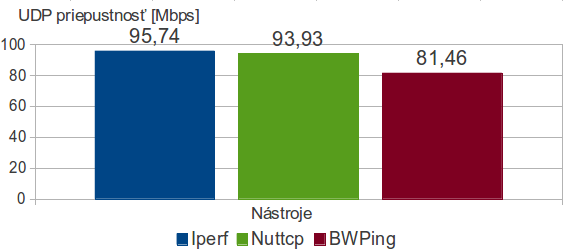
\includegraphics{img/cz_udp.png}}
               \caption{Graf odmeranej UDP priepustnosti testovaných nástrojov
               z~Brna.}
           \label{tab_test_udp_graf}
       \end{center}
   \end{figure}

%UDP SWISS
    \begin{table}[h!]
        \begin{center}
            \begin{tabular}{|c|c|c|c|}
                \hline
                Nástroj & Iperf [Mbps]&
                    Nuttcp [Mbps] & BWPing [Mbps] \\ 
                \hline
                1.beh o~00:00 & 0,22 & 0,22 & 0,21 \\
                \hline
                2.beh o~06:00 & 0,19 & 0,22 & 0,20 \\
                \hline
                3.beh o~12:00 & 0,22 & 0,22 & 0,19 \\
                \hline
                4.beh o~18:00 & 0,21 & 0,22 & 0,20 \\
                \hline
                priemer       & 0,21 & 0,22 & 0,20 \\
                \hline
                smerodajná odchýlka & \multicolumn{3}{c|}{0,008}\\
                %√((1÷3)×((0.21−0.21)²+(0.22−0.21)²+(0.20−0.21)²))
                \hline
            \end{tabular}
            \caption{Odmeraná UDP priepustnosť testovaných nástrojov
                zo~Švajčiarska.} 
            \label{tab_test_udp_swiss}
        \end{center}
    \end{table}
   \begin{figure}[H]
       \begin{center}
               \scalebox{0.67}{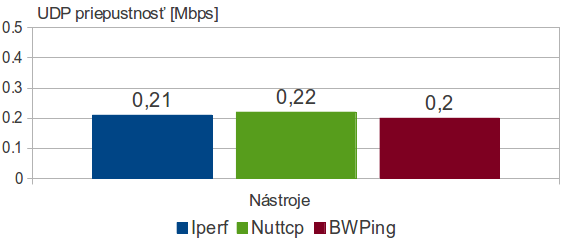
\includegraphics{img/swiss_udp.png}}
               \caption{Graf odmeranej UDP priepustnosti testovaných nástrojov
               zo Švajčiarska.}
           \label{tab_test_udp_swiss_graf}
       \end{center}
   \end{figure}

%UDP SK
    \begin{table}[h!]
        \begin{center}
            \begin{tabular}{|c|c|c|c|}
                \hline
                Nástroj & Iperf [Mbps]&
                    Nuttcp [Mbps] & BWPing [Mbps] \\ 
                \hline
                1.beh o~00:00 & 3,28 & 3,11 & 2,78 \\
                \hline
                2.beh o~06:00 & 3,10 & 2,93 & 2,95 \\
                \hline
                3.beh o~12:00 & 3,08 & 2,91 & 3,04 \\
                \hline
                4.beh o~18:00 & 3,10 & 2,94 & 2,13 \\
                \hline
                priemer       & 3,14 & 2,97 & 2,73 \\
                \hline
                smerodajná odchýlka & \multicolumn{3}{c|}{0,168}\\
                \hline
            \end{tabular}
            \caption{Odmeraná UDP priepustnosť testovaných nástrojov zo
                Slovenska.} 
            \label{tab_test_udp_sk}
        \end{center}
    \end{table}
   \begin{figure}[H]
       \begin{center}
               \scalebox{0.67}{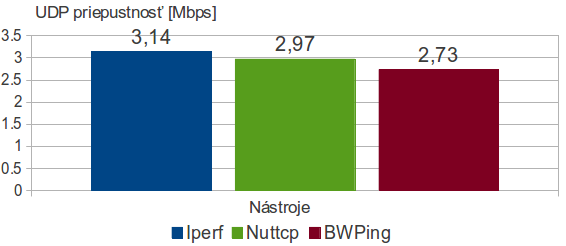
\includegraphics{img/sk_udp.png}}
               \caption{Graf odmeranej UDP priepustnosti testovaných nástrojov
               zo Slovenska.}
           \label{tab_test_udp_sk_graf}
       \end{center}
   \end{figure}

   \newpage
        \subsection{Strata paketov} \label{test_vys_strata}
        Výsledky stratovosti paketov sú uvedené v~tabuľke \ref{tab_test_loss}
        pre Brno, \ref{tab_test_loss_sk} pre Slovensko
        a~\ref{tab_test_loss_swiss} pre Švajčiarsko. Pre prehľadnosť uvádzame
        tabuľku \ref{vys_loss}, ktorá obsahuje výsledky nameranej stratovosti
        v~percentách, odmeranej a~nastavenej priepustnosti.

        Z~výsledkov je zrejmé, že ak nastavená hodnota maximálnej testovanej 
        priepustnosti je väčšia ako reálne dosiahnutá, tak sa stratovosť paketov 
        zväčší. Preto pri testovaní UDP priepustnosti doporučujeme vhodne zvoliť
        maximálnu priepustnosť, aby stratovosť nebola príliš veľká.

        Výsledky meraní z~Brna ukazujú, že výsledná hodnota stratovosti
        paketov je 0,00 \% pre všetky nástroje. Nastavená hodnota testovanej
        priepustnosti bola 100 Mbps a~dosiahnutá hodnota 90,38 Mbps. Nulová
        stratovosť je príčinou kvalitnej akademickej siete. Meranie 
        nepreukázalo priepustnosť 100 Mbps. Tá je len teoretická, pretože 
        klientská stanica disponuje sieťovou kartou s~maximálnou rýchlosťou 100
        Mbps.
        
        Výsledky z~ďalších dvoch destinácii ukazujú porovnateľné výsledky
        nástrojov. Smerodajné odchýlky vyšli 0,977 pre Švajčiarska
        a~1,996 pre Slovensko. Tieto hodnoty poukazujú na to, že všetky testované
        nástroje odmerali približne rovnakú stratovosť pri nastavenej maximálnej 
        priepustnosti.
        Z~tohto môžeme usúdiť, že ľubovoľný z~vybraných nástrojov je 
        vhodný na meranie stratovosti paketov.

        \begin{table}[h!]
            \begin{center}
                \begin{tabular}{|m{2cm}|m{3,2cm}|m{3,4cm}|m{3,4cm}|}
                    \hline
                    \multicolumn{1}{|c|}{Miesto} & Priemerná stratovosť paketov [\%] &
                    Nastavená UDP priepustnosť [Mbps] & 
                    Nameraná UDP priepustnosť [Mbps] \\  
                    \hline
                    \multicolumn{1}{|c|}{Brno} & \multicolumn{1}{c}{0,00} & 
                        \multicolumn{1}{|c|}{100,00} & \multicolumn{1}{c|}{90,38} \\
                    \hline
                    \multicolumn{1}{|c|}{Slovensko} & \multicolumn{1}{c}{13,71} & 
                        \multicolumn{1}{|c|}{3,50} & \multicolumn{1}{c|}{2,95} \\
                    \hline
                    \multicolumn{1}{|c|}{Švajčiarsko} & \multicolumn{1}{c}{84,04} & 
                        \multicolumn{1}{|c|}{2,00} & \multicolumn{1}{c|}{0,21} \\
                    \hline
                \end{tabular}
                \caption{Výsledky stratovosti paketov.} 
                \label{vys_loss}
            \end{center}
        \end{table}

%LOSS CZ
    \begin{table}[h!]
        \begin{center}
            \begin{tabular}{|c|c|c|c|c|c|}
                \hline
                Nástroj & Iperf [\%]&  Thrulay [\%]& Nuttcp [\%]\\ 
                \hline
                1.beh o~00:00 & 0,00  & 0,00 & 0,00 \\
                \hline
                2.beh o~06:00 & 0,00 & 0,00 & 0,00 \\
                \hline
                3.beh o~12:00 & 0,00 & 0,00 & 0,00 \\
                \hline
                4.beh o~18:00 & 0,00 & 0,00 & 0,00 \\
                \hline
                priemer & 0,00 & 0,00 & 0,00 \\
                \hline
                smerodajná odchýlka & \multicolumn{3}{c|}{0,00}\\
                \hline
            \end{tabular}
            \caption{Odmeraná strata paketov testovaných nástrojov z~Brna.} 
            \label{tab_test_loss}
        \end{center}
    \end{table}
%   \begin{figure}[H]
%       \begin{center}
%               \scalebox{0.75}{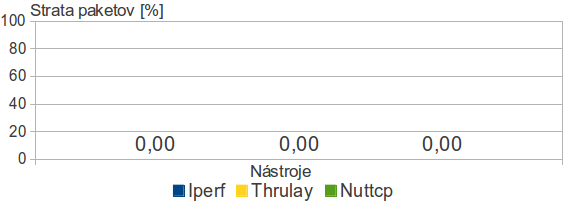
\includegraphics{img/cz_loss.png}}
%               \caption{Graf odmeranej stratovosti paketov z~Brna.}
%           \label{tab_test_loss_graf}
%       \end{center}
%   \end{figure}

%LOSS Swiss
    \begin{table}[h!]
        \begin{center}
            \begin{tabular}{|c|c|c|c|}
                \hline
                Nástroj & Iperf [\%]&  Thrulay [\%]& Nuttcp [\%]\\ 
                \hline
                1.beh o~00:00 & 83,36 & 82,72 & 85,15 \\
                \hline
                2.beh o~06:00 & 85,41 & 82,69 & 85,15 \\
                \hline
                3.beh o~12:00 & 83,44 & 82,71 & 85,17 \\
                \hline
                4.beh o~18:00 & 84,56 & 82,98 & 85,16 \\
                \hline
                priemer       & 84,19 & 82,78 & 85,16 \\
                \hline
                smerodajná odchýlka & \multicolumn{3}{c|}{0.977}\\
                %√((1÷3)×((84.19−84.04)²+(82.78−84.04)²+(85.16−84.04)²))
                \hline
            \end{tabular}
            \caption{Odmeraná strata paketov testovaných nástrojov zo~Švajčiarska.} 
            \label{tab_test_loss_swiss}
        \end{center}
    \end{table}
   \begin{figure}[H]
       \begin{center}
               \scalebox{0.67}{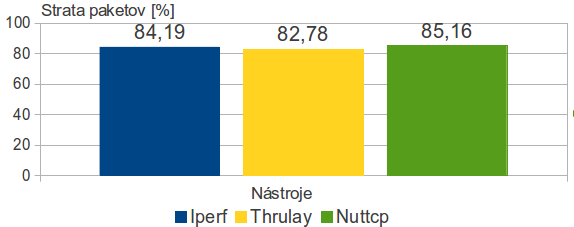
\includegraphics{img/swiss_loss.png}}
               \caption{Graf odmeranej stratovosti paketov zo Švajčiarska.}
           \label{tab_test_loss_swiss_graf}
       \end{center}
   \end{figure}

%LOSS SK
    \begin{table}[h!]
        \begin{center}
            \begin{tabular}{|c|c|c|c|}
                \hline
                Nástroj & Iperf [\%]&  Thrulay [\%]& Nuttcp [\%]\\ 
                \hline
                1.beh o~00:00 & 9,90 & 14,04 & 14,27 \\
                \hline
                2.beh o~06:00 & 11,23 & 14,10 & 16,07 \\
                \hline
                3.beh o~12:00 & 11,79 & 14,78 &  16,92 \\
                \hline
                4.beh o~18:00 & 11,24 & 14,09 & 16,08 \\
                \hline
                priemer       & 11,04 & 14,25 & 15,84 \\
                \hline
                smerodajná odchýlka & \multicolumn{3}{c|}{1,996}\\
                \hline
            \end{tabular}
            \caption{Odmeraná strata paketov testovaných nástrojov zo Slovenska.} 
            \label{tab_test_loss_sk}
        \end{center}
    \end{table}
   \begin{figure}[H]
       \begin{center}
               \scalebox{0.67}{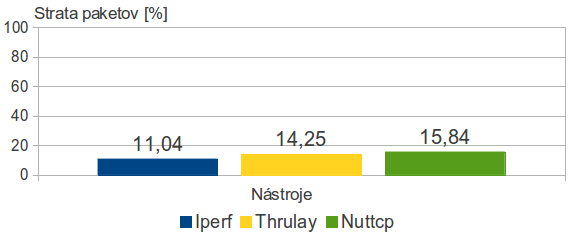
\includegraphics{img/sk_loss.png}}
               \caption{Graf odmeranej stratovosti paketov zo Slovenska.}
           \label{tab_test_loss_sk_graf}
       \end{center}
   \end{figure}

        \subsection{Jednosmerné oneskorenie} \label{test_vys_ones}
        Výsledky z~merania jednosmerného oneskorenia pomocou nástroja OWAMP sa
        nachádzajú v~tabuľke \ref{tab_test_delay}. Hodnota RTT by mala byť približne 
        rovná dvojnásobku hodnoty jednosmerného oneskorenia. Nemusí to platiť
        v~prípade, ak sú linky v~oboch smeroch rôzne zaťažené, alebo majú
        rozdielnu maximálnu prenosovú rýchlosť. Prípadne sa paket pošle inou
        cestou. Viacmenej hodnota RTT by mala byť vždy väčšia, ako hodnota
        jednosmerného oneskorenia.
        
        Výsledky merania ukazujú, že hodnota
        získaná pomocou utility OWAMP je väčšia, ako hodnota RTT utility Ping.
        Aby sme mohli presne určiť, ktorý z~nástrojov dáva presnejšie výsledky,
        je potrebné podrobnejšie a~rozsiahlejšie testovanie. Toto však nie je 
        predmetom našej práce.

%OWAMP
    \begin{table}[h!]
        \begin{center}
            \begin{tabular}{|c|c|c|}
                \hline
                Nástroj & OWAMP [ms]& Ping [ms] (RTT)\\ 
                \hline
                1.beh o~00:00 & 0,83 & 0,50 \\
                \hline
                2.beh o~06:00 & 0,52 & 0,49 \\
                \hline
                3.beh o~12:00 & 0,80 & 0,51 \\
                \hline
                4.beh o~18:00 & 0,90 & 0,52 \\
                \hline
                priemer & 0,76 & 0,51 \\
                \hline
            \end{tabular}
            \caption{Jednosmerné oneskorenie z~Brna.} 
            \label{tab_test_delay}
        \end{center}
    \end{table}
   \begin{figure}[H]
       \begin{center}
               \scalebox{0.67}{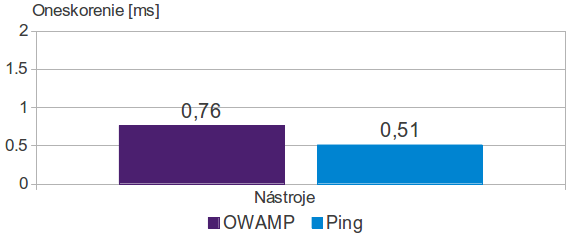
\includegraphics{img/cz_owamp.png}}
               \caption{Graf jednosmerného oneskorenia z~Brna.}
           \label{tab_test_delay_graf}
       \end{center}
   \end{figure}

   \section{Záver s~doporučením} \label{test_zaver}
    Výsledkom tejto kapitoly má byť doporučenie pre bežného užívateľa, aby
    vedel, ktorý nástroj má použiť na meranie vybraného parametra sieťového
    prenosu. Tabuľka \ref{tab_zhod_param} obsahuje informácie o~funkcionalite nástrojov
    pre meranie rôznych parametrov sieťového prenosu.
    My sme sa zamerali na overenie funkcionality nástrojov pre meranie 
    priepustnosti pod oboma transportnými protokolmi TCP a~UDP, stratu
    paketov a~jednosmerného oneskorenia.

    Merania v~tejto kapitole
    ukázali, že všetky z~nástrojov sú schopné odmerať vybrané parametere. Rozdiely
    vo výsledkoch boli minimálne. Preto výber najvhodnejšieho nástroja bude
    záležať na funkcionalite a~možnostiach použitia. Taktiež treba brať v~úvahu
    dostupnosť nástroja v~balíčkových systémoch a~nami nájdené nekorektné chovanie.

    Pre meranie TCP priepustnosti by sme mohli zvoliť ľubovoľný z~testovaných 
    nástrojov, pretože všetky odmerali viac menej rovnaké hodnoty.
    Ak by sme mali vybrať nástroj, ktorý sa jednoducho používa, je dostupný
    a~poslúži aj na meranie ostatných parametrov, bol by to Iperf a~Nuttcp.
    Utilita Iperf je v~súčasnej dobe najrozšírenejšia. Nájdeme ju
    skoro vo všetkých balíčkových repozitároch. Druhý zmienený nástroj je
    výhodnejšie kompilovať zo zdrojových textov, pretože sa stále
    vyvíja.

    Na merania UDP priepustnosti máme na výber tri nástroje: Iperf, Nuttcp
    a~BWPing. Posledná utilita nebola schopná správne odmerať priepustnosť. 
    Namerané hodnoty boli vždy menšie v~porovnaní s~ostatnými nástrojmi. Pre
    tieto fakty a~problémy s~ICMP správami doporučujeme používať
    tento nástroj v~prípade, ak nemáme prístup na druhú stanicu. Namerané
    hodnoty však nebudú korektné. Odporúčaný nástroj pre meranie UDP
    priepustnosti je Nuttcp
    a~Iperf. Pri nástroji Iperf treba spomenúť nekorektné správanie, v~ktorom
    klientská časť aplikácie niekedy nezobrazí namerané hodnoty serverovej časti. 
    Toto sa prejavuje iba pri meraní UDP priepustnosti.
    Výsledky sa však zobrazia na štandardnom výstupe servera.

    Stratovosť paketov úzko súvisí s~meraním UDP priepustnosti. Pri
    tomto druhu teste máme k~dispozícii informácie o~stratovosti. Odporúčané nástroje
    by boli opäť Iperf a~Nuttcp. Utilitu Thrulay nedoporučujeme, pretože neposkytuje 
    informáciu o~nameranej priepustnosti.

    Ak by sme mali vybrať nástroj, ktorý dokáže odmerať všetky vybrané parametre
    sieťového prenosu, bol by to Nuttcp. Je veľmi jednoduchý na ovládanie, ale
    jeho aktuálna verzia sa nenachádzala v~balíčkových repozitároch.
    Druhým najpoužiteľnejším nástrojom 
    je Iperf. Je jednoduchý na použitie
    a~jeho schopnosti merania sú rovnaké ako u~Nuttcp. Jeho hlavnou prednosťou je 
    dostupnosť aktuálnej verzie v~balíčkových repozitároch. 

    Posledné meranie sa venovalo overeniu výsledkov nástroja OWAMP. Tento
    nástroj vždy odmeral hodnotu jednosmerného oneskorenia väčšiu oproti hodnote
    RTT. Výsledky sa priemerne líšili o~0.25 ms, čo je pomerne malá hodnota.
    Aby sme mohli rozhodnúť, ktorý nástroj poskytuje správne výsledky, vyžadovalo by to
    podrobnejšie merania.
    Treba
    zdôrazniť, že aplikácia Ping je dostupná vo väčšine systémov, oproti
    nástroju OWAMP, ktorý vyžaduje kompiláciu zo zdrojových textov
    a~synchronizovaný čas pomocou NTP. Po zvážení týchto faktorov je 
    jednoduchšie použiť utilitu Ping.

\chapter{Záver}
    V~našej práci sme sa zaoberali porovnávaním a~testovaním open source
    nástrojov na meranie rôznych parametrov sieťového prenosu. Pre bližšie
    pochopenie, akým spôsobom sa merajú tieto parametre, sme uviedli metodiky, 
    ktoré sa touto činnosťou zaoberajú. Tento krok nám taktiež pomohol k~vytvoreniu 
    metodiky na porovnanie nástrojov na báze funkcionality.

    Hlavnou úlohou práce bolo testovanie nástrojov na reálnej sieti. Pre
    účely testovania bola vytvorená metodika, v~ktorej sme stanovili, aké 
    parametre prenosu budeme sledovať a~za akých podmienok. Výsledky meraní
    sme analyzovali a~nástroje medzi sebou druhý krát porovnali. V~tomto kroku sme
    sa zamerali na rozdiely nameraných hodnôt. Výsledkom merania bolo určenie
    vhodného nástroja na meranie daného parametra sieťového prenosu. Pri
    určovaní vhodného nástroja sme brali do úvahy aj chybné správanie a~ďalšie
    funkcionálne vlastnosti nástrojov.

    Zo získaných informácií a~výsledkov meraní sme vytvorili
    webové stránky\footnote{Dostupné na \url{https://nes.fit.vutbr.cz/ansa/pmwiki.php?n=Main.Xloffa00}}.
    Obsahujú popisy jednotlivých utilít, ich
    funkcionálne schopnosti a~doporučenie, ktorý nástroj je vhodný na meranie
    daného parametra sieťového prenosu.

    Z~analýzy metodiky na meranie priepustnosti je jasné, že je potrebný softvér
    typu \mbox{klient\,--\,server.} To spôsobuje pre bežného užívateľa
    problém, pretože väčšinou nemá k~dispozícii druhú koncovú stanicu s~verejnou
    IP adresou, na ktorej by mohol nástroj nainštalovať. Toto by mohli zabezpečiť 
    poskytovatelia pripojenia na ich serveroch. 
    
    Mnohokrát sa samotní klienti
    sťažujú poskytovateľovi služieb na \czuv{pomalé pripojenie}. ISP však nie
    je schopný odmerať priepustnosť voči klientovi. Tu nastáva priestor pre
    implementáciu softvéru, ktorý by bol umiestnený v~aktívnom sieťovom
    zariadení, ktoré je pod správou ISP, ale umiestnené u~klienta. Táto utilita
    by zabezpečovala meranie priepustnosti, straty paketov a~iných parametrov
    potrebných pre diagnostiku pripojenia. Takto by sa poskytovateľ pripojenia
    mohol brániť pred sťažovaním klienta. Taktiež by to
    viedlo k~rýchlejšej identifikácii závady. Táto aplikácia by mnohým
    užívateľom vyriešila problém merania parametrov sieťového prenosu. 

 % viz. obsah.tex

  % Pouzita literatura
  % ----------------------------------------------
  % \bibliographystyle{czechiso}
\ifczech
  \bibliographystyle{czplain}
\else 
  \bibliographystyle{czplain}
%  \bibliographystyle{alpha}
\fi
  \begin{flushleft}
  \bibliography{literatura} % viz. literatura.bib
  \end{flushleft}
  \appendix
  
  %\chapter{Obsah CD}
%\chapter{Manual}
%\chapter{Konfigrační soubor}
%\chapter{RelaxNG Schéma konfiguračního soboru}
%\chapter{Plakat}

\chapter{Obsah CD disku}
    \begin{itemize}
        \item Zdrojový kód technickej správy v adresári \texttt{sprava}
        \item Skript pre spúšťanie automatizovaného testovania v adresári
            \texttt{test}
        \item Zdrojový kód webovej stránky v adresári \texttt{www}.    
        \item Návod na použitie v súbore \texttt{readme.txt}
    \end{itemize}
 % viz. prilohy.tex
\end{document}
